\documentclass[norsk,a4paper,12pt]{scrartcl}
\usepackage[T1]{fontenc} %for å bruke æøå
\usepackage[utf8]{inputenc}
\usepackage{graphicx} %for å inkludere grafikk
\usepackage{verbatim} %for å inkludere filer med tegn LaTeX ikke liker
\usepackage{mathpazo}
\usepackage{amsfonts,amsthm}
\usepackage{amsmath}
\usepackage{float}
\usepackage[english]{babel}
\usepackage{listings}
\usepackage{biblatex}
\usepackage[noend]{algpseudocode}
%\usepackage[style=numeric]{biblatex}
%\usepackage{comment}
\addbibresource{Reference.bib}
\usepackage{subcaption}
\usepackage{listings}
\usepackage{caption}
\usepackage{subcaption}
\usepackage{siunitx}
\usepackage{mathtools}
\usepackage[table,xcdraw]{xcolor}
\usepackage{hyperref}
\usepackage[linesnumbered,ruled,vlined,lined,boxed,commentsnumbered]{algorithm2e}
\usepackage{float}
\newcommand{\Lagr}{\mathcal{L}}
\renewcommand\qedsymbol{$\blacksquare$}
\DeclareMathOperator*{\E}{\mathbb{E}}
\hypersetup{
    colorlinks=true,
    linkcolor=blue,
    filecolor=magenta,      
    urlcolor=cyan,
}

\urlstyle{same}


\renewcommand{\vec}[1]{\mathbf{#1}} % \vec gives bold text instead of arrow


% For changing linespacing in matrices
\makeatletter
\renewcommand*\env@matrix[1][\arraystretch]{%
  \edef\arraystretch{#1}%
  \hskip -\arraycolsep
  \let\@ifnextchar\new@ifnextchar
  \array{*\c@MaxMatrixCols c}}
\makeatother


%\title{Exploring the complex many body system of our solar system}
\begin{document}
\title{Project 1, Regression analysis and resampling methods}
\date{\today}

\author{Sakarias Frette, Mikkel Metzsch-Jensen, William Hirst}
\maketitle
\begin{abstract}
    The code for this project is at \href{https://github.com/Gadangadang/Fys-Stk4155/tree/main/Project\%201}{this Github adress}. Please read the ReadME file before running the code.
\end{abstract}

\newpage

\tableofcontents

\newpage
\section{Introduciton and general method}
In this project we will study the Franke's Function f(x, y) in the domain $x,y \in [0,1]$. Franke's function, which is a weighted sum of four exponentials, reads as follows
\begin{align*}
f(x,y) &= \frac{3}{4}\exp{\left(-\frac{(9x-2)^2}{4} - \frac{(9y-2)^2}{4}\right)}+\frac{3}{4}\exp{\left(-\frac{(9x+1)^2}{49}- \frac{(9y+1)}{10}\right)} \\
&+\frac{1}{2}\exp{\left(-\frac{(9x-7)^2}{4} - \frac{(9y-3)^2}{4}\right)} -\frac{1}{5}\exp{\left(-(9x-4)^2 - (9y-7)^2\right) }.
\end{align*}
We generate data from this function by adding stochastic noise. In practice the noise is computed by drawing points from a normal distribution with mean $\mu=0$ and variance $\sigma^2$. We discretize the x,y data points in a $N \times N$ mesh-grid such that we get $N^2$ uniform distributed points in the space $x,y \in [0,1]$. The target value $z$ is then generated as follows
\begin{align*}
    z(x,y) = f(x,y) + N(0,\sigma^2).
\end{align*}

\subsection{Scaling}
For every data set one should consider whether it is nessecary to scale the data. Hence we investigate the behaviour of the Franke's function in our domain $x,y \in [0,1]$. For a quick judgment we take a look at the 3D plot as showed in figure \ref{fig:Franke3D}.
\begin{figure}[H]
    \centering
    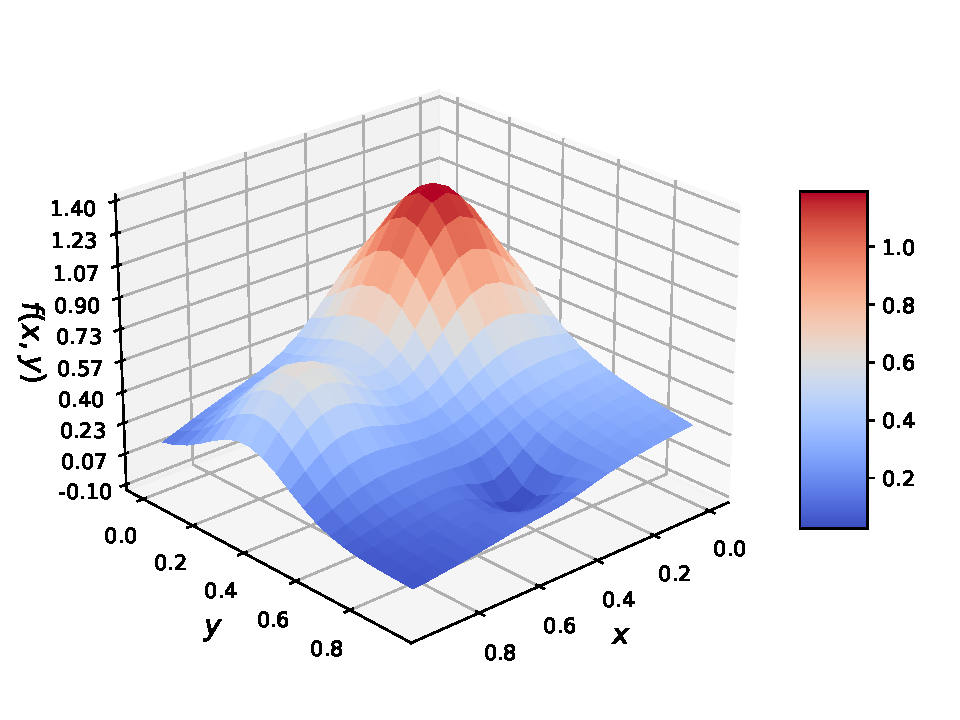
\includegraphics[width = \linewidth]{figures/Frankefunction_3D.pdf}
    \caption{A 3D plot of Franke's function $f(x,y)$ in the relevant domain of $x,y \in [0,1]$. For this plot we used a grid spacing of 0.05.}
    \label{fig:Franke3D}
\end{figure}
From figure \ref{fig:Franke3D} we see that our data is already quite "well-behaved". By making an even finer discretization than used in figure \ref{fig:Franke3D}, with $dx, dy = 10^{-4}$, we compute the minimum and maximum value for $z$ within our domain:
\begin{align*}
    \min{z} &= 0.011, \\
    \max{z} &= 1.220. 
\end{align*}
We observe that the target values are already very close to the [0,1]-range which is a common range to scale for. Since the x,y-values already lies within the [0,1]-range it should not be necessary to scale the data by any scaling-factors. In fact if we divide by the standard deviation, we will increase the variance in the dataset since the standard deviation is less than one in this case. However, since there might be some benefit of scaling by the mean (especially for Lasso regression), we shall do this consistently throughout the exercises involving Franke's function in order to compare the results. That is, we scale the design matrix and the target values by subtracting the mean. When generating predictions one should add back the mean value subtracted in the beginning. Note that we scale train and test data individually to avoid adding any further correlations.

\subsubsection{Fitting of the function}
In this project we will fit polynomials of different degree to Franke's function. Since we have two input variables $(x,y)$ a polynomial of degree $n$ will refer to every combination of $x^iy^j$ for which $i+j \le n$. 
For a polynomial of $n = 2$ our model $\tilde{z}$ will read:
\begin{align*}
    \tilde{z}(x,y)_{n=2} = \beta_0 + \beta_1x + \beta_2y +  + \beta_3x^2 + \beta_4xy + \beta_5y^2.
\end{align*}
We implement our polynomial model in the form of a design matrix $X$. We assign each term from the polynomial to the columns $X$, such that we for the $n = 2$ case get
\begin{align*}
\vec{X}_{n=2} = 
    \begin{bmatrix}[1.8]
        1 & x_0 & y_0  & x_0^2 & x_0y_0 & y_0^2 \\
        1 & x_1 & y_1  & x_1^2 & x_1y_1 & y_1^2 \\
        \vdots & \vdots & \vdots & \vdots & \vdots & \vdots   \\
        1 & x_{N-1} & y_{N-1} & x_{N-1}^2 & x_{N-1}y_{N-1} & y_{N-1}^2
    \end{bmatrix}
    , \quad \beta = 
    \begin{bmatrix}[1.8]
        \beta_0  \\
        \beta_1 \\
        \vdots  \\
        \beta_{N-1}
    \end{bmatrix}.
\end{align*}
Notice that the design matrix in general have dimensions $(N^2 \times (n+1)(n+2)/2$, as we have $N^2$ points in the meshgrid and $(n+1)(n+2)/2$ terms in our polynomial model. This means that we have to flatten the meshgrid of the $x_i,y_j$ index-combinations into a vector suitable for the columns of the design matrix. Notice that the first column in the design matrix will be scaled to zero when subtracting the mean of every column, and thus this is effectively left out of the regression. By implementing the design matrix our polynomial model can be represented as
\begin{align*}
     \tilde{z}(x,y) = \vec{X}\beta.
\end{align*}
\subsubsection{Splitting of data}
When working with fitting of data it is essential and customary to distribute the data into training and test data. We choose to use a 80-20 split, meaning that we use 80\% of the data for our regression model (training) and 20\%  of the data, which is unseen for the model, to evaluate the model predictions (test).


\subsubsection{Notation}
We will not distinct matrices and vectors in the notation as we write both with bold letters throughout the paper. However, in many situations the bold letters just make the notations more cluttered and when left out we expect the presence of vectors and matrices to be clear from the context.


\newpage
\section{Exercise 1}\label{sec:exer1}
First we perform Ordinary Least Squares (OLS) regression using polynomials up to fifth order ($n=5$). In short, we define the OLS regression as a minimization of the cost function
\begin{align*}
    C(\vec{X}, \boldsymbol{\beta})=\frac{1}{n} \sum_{i=0}^{n-1}\left(z_{i}-\tilde{z}_i\right)^{2}=
    \frac{1}{n}\left[(\boldsymbol{z}-\boldsymbol{\tilde{z}})^{T}(\boldsymbol{z}-\boldsymbol{\tilde{z}})\right], \qquad \vec{\tilde{z}} = \vec{X}\boldsymbol{\beta}.
\end{align*}

By taking the derivative and setting it equal to zero, one can show that the optimal $\beta$-parameters is found as
\begin{align*}
    \hat{\boldsymbol{\beta}} = (\vec{X}^T\vec{X})^{-1}\vec{X}^T\vec{z}.
\end{align*}
In addition one will get that the variance of the $\beta$-parameters $\beta_i$ is given as the diagonal elements
\begin{align*}
    \text{diag}\Big(\text{var}(\hat{\beta}_0),\ \text{var}(\hat{\beta}_1),\ \hdots,\ \text{var}(\hat{\beta}_{n-1})\Big) = (\vec{X}^T\vec{X})^{-1} ,
\end{align*}
for which we can calculate the standard error as $SE(\hat{\beta}_i) = \sqrt{\text{var}(\hat{\beta}_i)}$. \\
\\
By the use of the the above relations we perform OLS with polynomials with $n=5$ for a $N\times N$ grid with $N = 25$ (625 points) and added noise with $\sigma = 0.2$. Using the standard error (SE) for $ \hat{\boldsymbol{\beta}}$, we can display the results with a 95\% confidence interval (assuming $\hat{\boldsymbol{\beta}}$ is standard distributed). The values of $ \hat{\boldsymbol{\beta}}$ and the confidence interval is displayed in both table $\ref{tab:beta_uncertainty}$ and figure \ref{fig:beta_uncertainty}. 

\begin{table}[H]
\begin{center}
\caption{$\hat{\beta}$-values for OLS regression with a polynomial of degree $n=5$ using $N = 25$ and $\sigma = 0.2$. The uncertainty is the result of a $95\%$-confidence interval.}
\begin{tabular}{|c|c|c|} \hline
 \text{Beta} & \text{Train uncertainty} & \text{Test uncertainty} \\\hline
0.00 & $\pm$0.00 & $\pm$0.00\\\hline
5.65 & $\pm$13.13 & $\pm$29.47\\\hline
1.81 & $\pm$14.54 & $\pm$22.35\\\hline
-24.09 & $\pm$66.03 & $\pm$143.70\\\hline
-4.26 & $\pm$54.08 & $\pm$104.16\\\hline
0.34 & $\pm$70.05 & $\pm$128.41\\\hline
29.92 & $\pm$151.83 & $\pm$325.09\\\hline
18.02 & $\pm$111.78 & $\pm$246.34\\\hline
0.98 & $\pm$121.01 & $\pm$198.55\\\hline
-24.75 & $\pm$156.09 & $\pm$315.61\\\hline
-8.95 & $\pm$159.61 & $\pm$347.41\\\hline
-28.55 & $\pm$120.98 & $\pm$256.76\\\hline
15.05 & $\pm$115.41 & $\pm$237.71\\\hline
-12.25 & $\pm$128.46 & $\pm$234.38\\\hline
42.30 & $\pm$162.12 & $\pm$341.77\\\hline
-2.93 & $\pm$62.38 & $\pm$140.52\\\hline
10.57 & $\pm$54.03 & $\pm$117.66\\\hline
2.80 & $\pm$52.20 & $\pm$123.58\\\hline
-13.29 & $\pm$53.70 & $\pm$118.11\\\hline
10.94 & $\pm$54.80 & $\pm$126.30\\\hline
-20.04 & $\pm$63.13 & $\pm$137.01\\\hline
\end{tabular}
\label{tab:beta_uncertainty}
\end{center}
\end{table}

\begin{figure}[H]
    \centering
    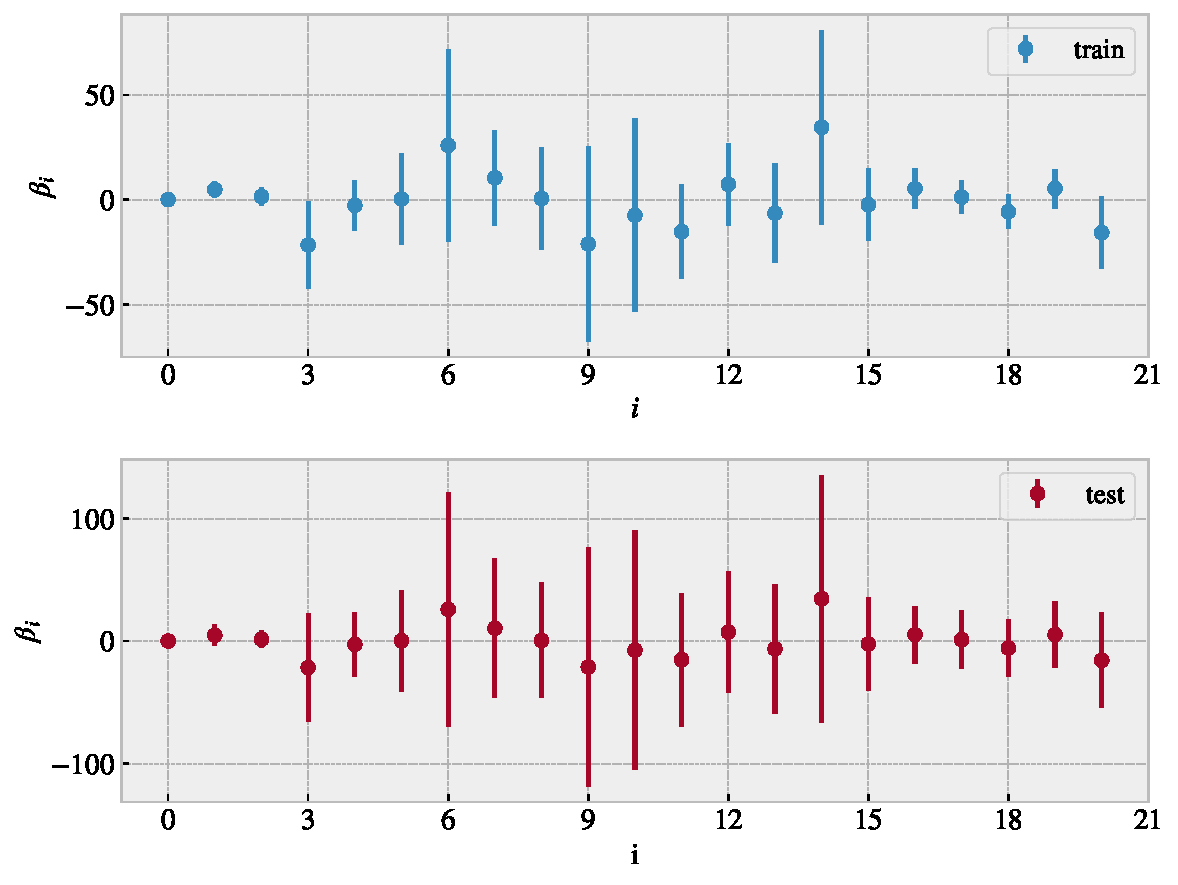
\includegraphics[width=\linewidth]{figures/confidence_interval.pdf}
    \caption{$\hat{\beta}$-values for OLS regression with a polynomial of degree $n=5$ using $N = 25$ and $\sigma = 0.2$. The uncertainty is the result of a $95\%$-confidence interval.}
    \label{fig:beta_uncertainty}
\end{figure}
From table \ref{tab:beta_uncertainty} and figure \ref{fig:beta_uncertainty} we see a noticeable difference in the uncertainty amplitude for different $\hat{\beta}_i$. Generally we have a bigger uncertainty for $\hat{\beta}_i$ with $i \approx [6,14]$, meaning that these $\hat{\beta}$-values have a higher variance. Also, since the test data is four times smaller than the training the data, we see as expected that the uncertainty is greater for the test data prediction. \par
\\
Lastly we can calculate the mean squared error (MSE) and $R^2$ score for our training and test data respectively as 
\begin{align*}
    \text{MSE}(\vec{z}, \vec{\tilde{z}})=\frac{1}{N^2} \sum_{i=0}^{N^2-1}\left(z_{i}-\tilde{z}_{i}\right)^{2},
\end{align*}
\begin{align*}
    R^{2}(\vec{z}, \vec{\tilde{z}})=1-\frac{\sum_{i=0}^{N^2-1}\left(z_{i}-\tilde{z}_{i}\right)^{2}}{\sum_{i=0}^{N^2-1}\left(z_{i}-\E(z)\right)^{2}}.
\end{align*}
where $\vec{z}$ is the input data and $\vec{\tilde{z}}$ is the model prediction. The error results from the $n=5$ OLS-regression is shown in table \ref{tab:n5_error}

\begin{table}[H]
  \begin{center}
  \caption{MSE and $R^2$ score for the test and train data on the OLS model. Using $n = 5$, $N = 25$ and $\sigma = 0.2$.}
  \begin{tabular}{|c|c|c|} \hline
  & \text{Train} & \text{Test}  \\
  \hline
  \text{MSE} & 0.045 & 0.050  \\ 
  \hline
   $\text{R}^2$ & 0.64 & 0.50  \\
  \hline
  \end{tabular}
  \label{tab:n5_error}
  \end{center}
\end{table}
As expected we see that the MSE for the training data is slightly better than MSE for the test data. This is because the model was trained to fit the train data and hence the fit is expected to be equal to or better than the fit on the test data.
%
%
%
\newpage
\section{Exercise 2}
In this exercise we aim to study the bias-variance tradeoff by implementing the bootstrap resampling technique.

\subsection{Error as a function of model complexity}
Before diving into the analysis we compute the training and test MSE for OLS regressions as a function of the complexity $n$. This let us identify possible regions of low and high bias and variance respectively. The result are shown in figure \ref{fig:hastie_copycat}.
\begin{figure}[H]
    \centering
    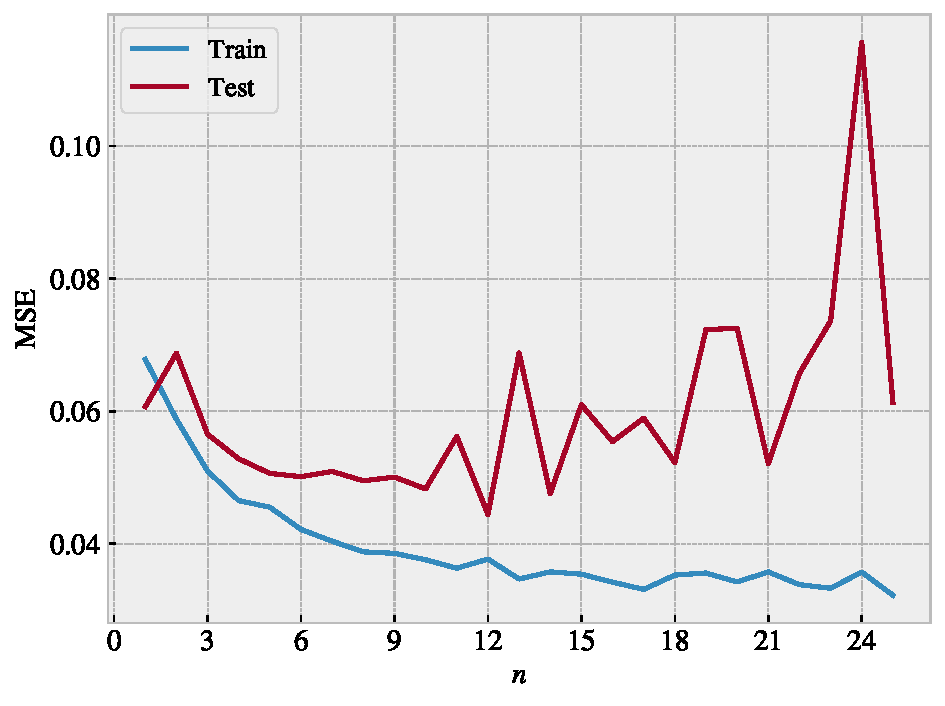
\includegraphics[width=0.7\linewidth]{figures/hastie_copycat.pdf}
    \caption{By performing OLS on the training data, we calculated the MSE between model predictions and input data for training and test data respectively. This was done as a function of the complexity $n$. We used $N = 25$ and $\sigma = 0.2$.}
    \label{fig:hastie_copycat}
\end{figure}
On figure \ref{fig:hastie_copycat} we see that the training MSE decreases steadily as the complexity increases, while the test MSE appears to be decreasing towards a minimum and then increasing again for higher complexities. This looks approximately similar to Fig. 2.11 of Hastie, Tibshirani, and Friedman, except for the fact that our results is a bit more rough. As expected the training MSE decreases as a function of the complexity since we make the model more and more adaptable to fit the training data. When the complexity gets to high, we will not only capture the general trend in the training data but also start fitting the model to the random noise applied to the training data. This does not translate well when using the model on the test data, and hence the predictions will start to deviate for higher complexities as we see. This is called overfitting. 
\pagebreak 
Judging from figure \ref{fig:hastie_copycat} the minimum test MSE sits around $n=12$, which indicate that a 12th-order polynomial is an appropriate model complexity to describe the general trend of Franke's function in our domain. \par 
In order to create a less noisy results that match Fig. 2.11 of Hastie, Tibshirani, and Friedman even better, we can repeat the complexity analysis multiple times by generating new data points each time (apply new random noise). Notice that this is normally not possible with limited data. But it serves a great point of showing the general trend of training and test MSE respectively regarding overfitting. The result is shown in figure \ref{fig:hastie_multi}.
\begin{figure}[H]
    \centering
    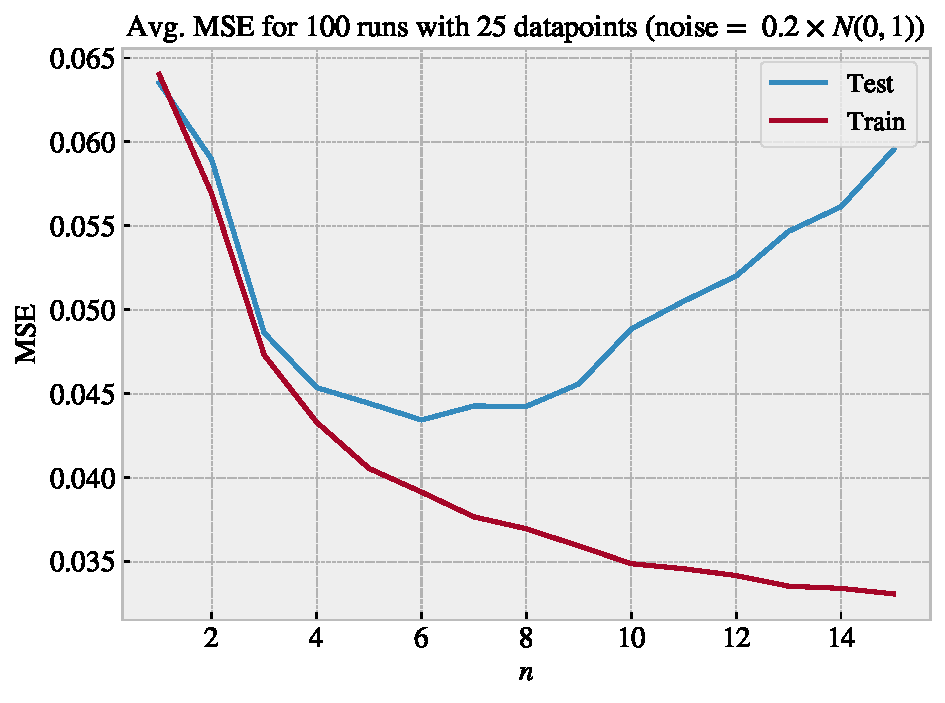
\includegraphics[width=0.8\linewidth]{figures/hastie_multi100.pdf}
    \caption{Average MSE for 100 repeatedly runs of the setup used for generating figure \ref{fig:hastie_copycat}. This averaged version highlights the general trend of the training and test MSE as the complexity increases.}
    \label{fig:hastie_multi}
\end{figure}
We see that the averaged result in figure \ref{fig:hastie_multi} resembles Fig. 2.11 of Hastie, Tibshirani, and Friedman even better.


\subsection{Visualization of the predictions}
In order to verify visually that our predictions is reasonable we plot the predictions on selected order of complexities. Hence we generate two complete data sets: training and test, both on size $N = 25$ and with applied noise of $\sigma = 0.2$. We then train the model on the training data using OLS and plot the model predictions on the test data. The results are shown in figure \ref{fig:z_multi}. We see that the predictions converge fairly good towards the expected trends of Franke's function. In addition we see visually that it agrees with the results on figure \ref{fig:hastie_multi}, which indicated that $n = 6$ might be the best complexity level. For $n = 20$ the prediction is clearly adding to many complex variations as a result to overfitting.
\begin{figure}[H]
     \centering
     \begin{subfigure}[b]{0.49\textwidth}
         \centering
         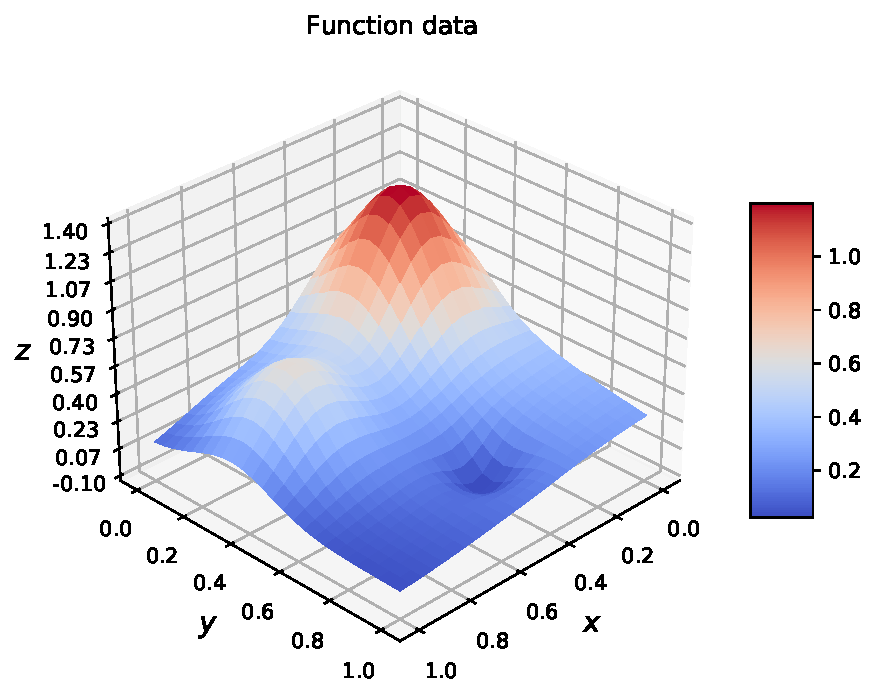
\includegraphics[width=\textwidth]{figures/zprediction/func_data.pdf}
         \caption{Franke's Function $f(x,y)$}
         \label{fig:z_func}
     \end{subfigure}
    \hfill
     \begin{subfigure}[b]{0.49\textwidth}
         \centering
         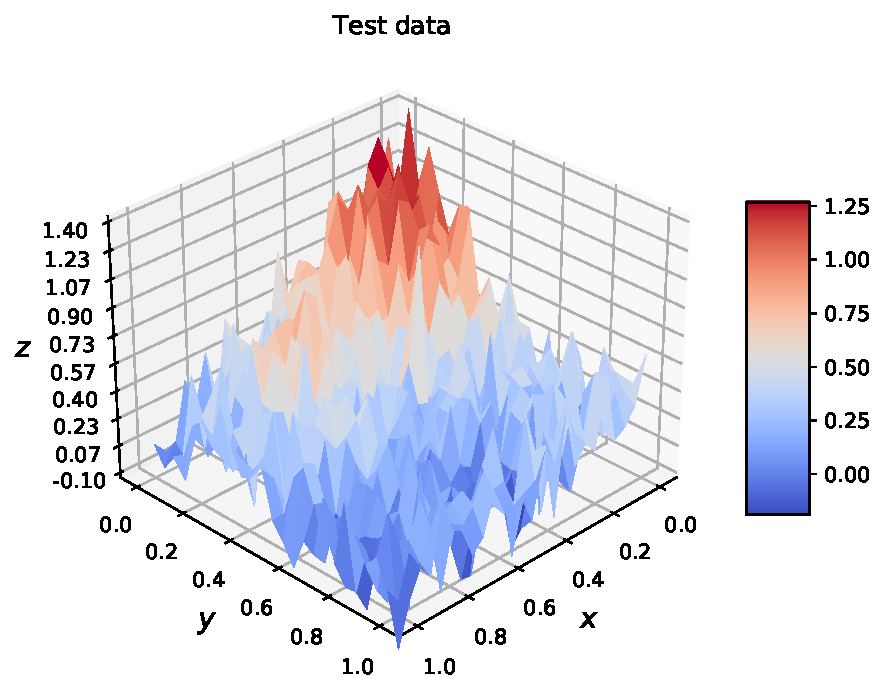
\includegraphics[width=\textwidth]{figures/zprediction/test_data.pdf}
         \caption{Test data $z = f(x,y) + \epsilon$ }
         \label{fig:z_test}
     \end{subfigure}
    \begin{subfigure}[b]{0.49\textwidth}
         \centering
         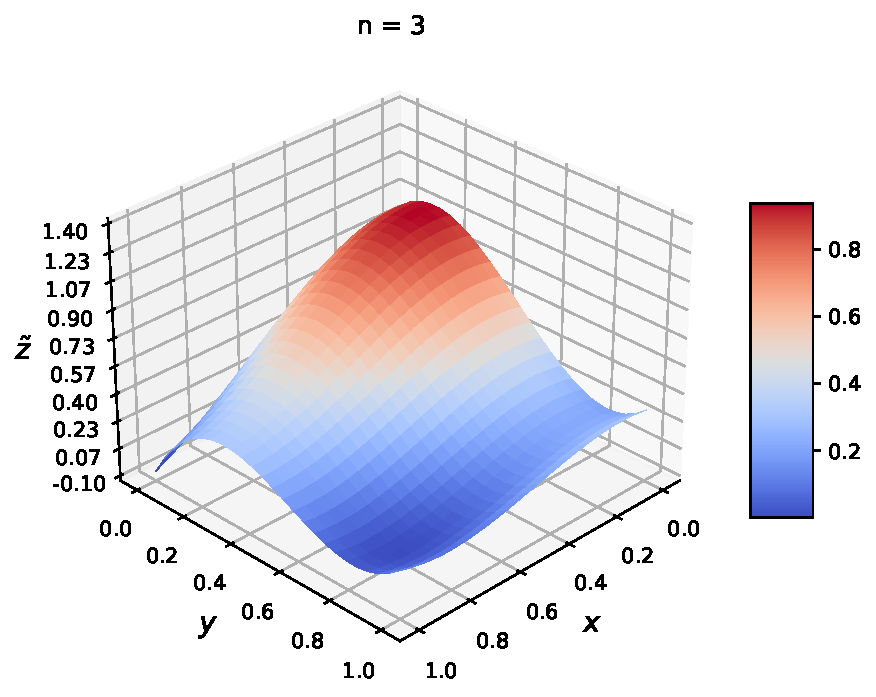
\includegraphics[width=\textwidth]{figures/zprediction/n3.pdf}
         \caption{Prediction $\tilde{z}$ for $n=3$}
         \label{fig:z_n3}
     \end{subfigure}
     \hfill
     \begin{subfigure}[b]{0.49\textwidth}
         \centering
         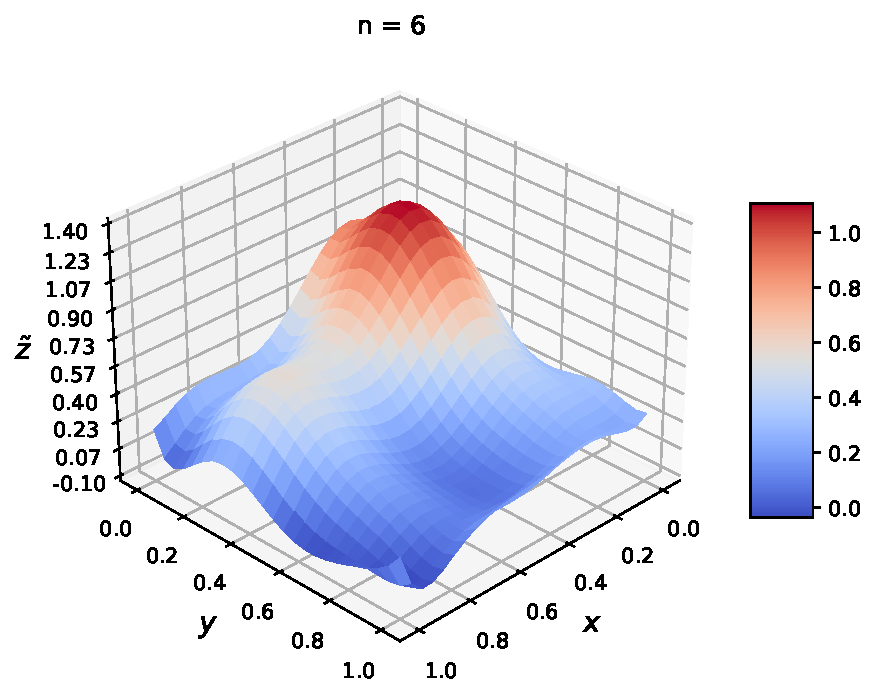
\includegraphics[width=\textwidth]{figures/zprediction/n6.pdf}
         \caption{Prediction $\tilde{z}$ for $n=6$}
         \label{fig:z_n6}
     \end{subfigure}
      \begin{subfigure}[b]{0.49\textwidth}
         \centering
         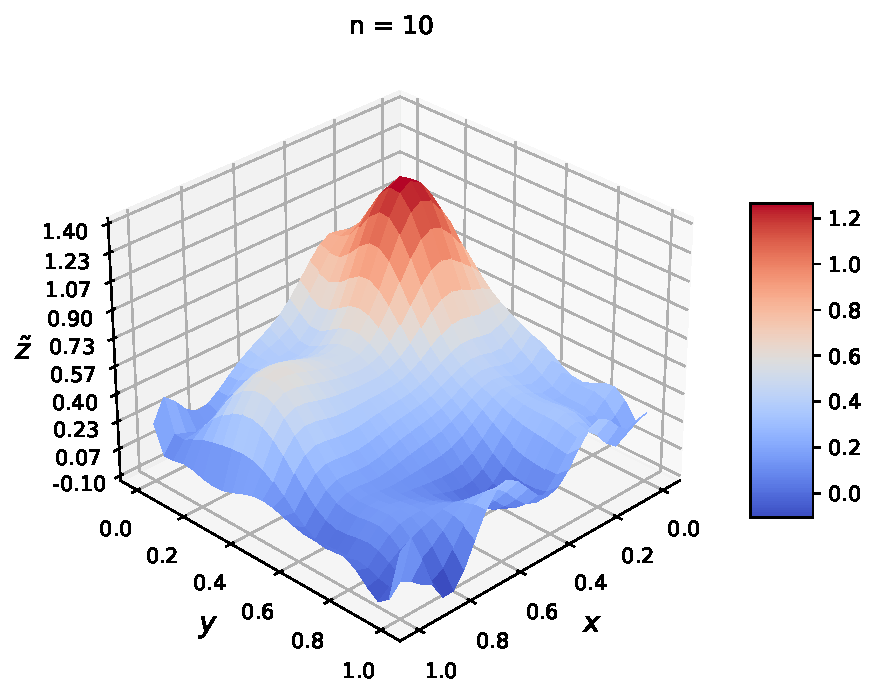
\includegraphics[width=\textwidth]{figures/zprediction/n10.pdf}
         \caption{Prediction $\tilde{z}$ for $n=10$}
         \label{fig:z_n10}
     \end{subfigure}
     \hfill
     \begin{subfigure}[b]{0.49\textwidth}
         \centering
         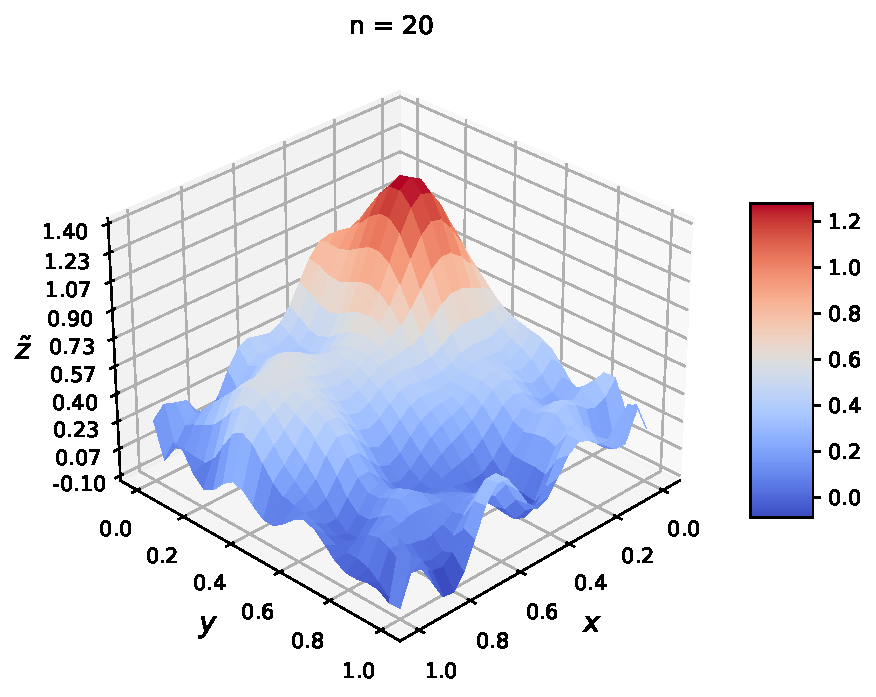
\includegraphics[width=\textwidth]{figures/zprediction/n20.pdf}
         \caption{Prediction $\tilde{z}$ for $n=20$}
         \label{fig:z_n20}
     \end{subfigure}
    \caption{Subfigure a and b show the Franke function with and without noise. Subfigures c through f show different OLS predictions for the Franke function with a given complexity.}
    \label{fig:z_multi}
\end{figure}


\subsection{Derivation of the Bias-Variance decomposition }\label{sec:bias_var_derivation}
We now move on to the Bias-Variance tradeoff analysis. We consider a general dataset $\Lagr$ which consists of the datapoints $\boldsymbol{X}_{\Lagr} = \{(y_j, \boldsymbol{X}_j), j=0, \hdots, n-1\}$. In this task we will assume that the true data is made from a model with normally distributed noise, with variance $\sigma^2$ and zero mean. Our model is thus 
\begin{equation}
    \Vec{y} = f(\boldsymbol{x}) + \boldsymbol\epsilon. 
\end{equation}
As previously stated, our model is given as $\tilde{\vec{y}} = \boldsymbol{X}\boldsymbol{\beta}$, where the optimal $\boldsymbol{\beta}$ is found as the minimization of the MSE cost function, which can also be written
\begin{equation}
    C(\vec{X},\boldsymbol{\beta}) = \frac{1}{n}\sum_{i=0}^{n-1} (y_i - \Tilde{y_i})^2 = \E [ (\Vec{y} - \Tilde{\Vec{y}})^2].
\end{equation}

We can decompose the MSE error into bias, variance and the noise variance. This is known as the Bias-Variance tradeoff. We have

\begin{equation*}
    \begin{aligned}
        \E [ (\Vec{y} - \Tilde{\Vec{y}})^2] = &\E [ ( f+\epsilon -\Tilde{y} )^2] \\
        = &\E [ ( f+\epsilon -\Tilde{y} + \E [\Tilde{y}] - \E [\Tilde{y}] )^2] \\
        = &\E [ f^2 + f\epsilon - \Tilde{y}f + f\E [\Tilde{y}] - f\E [\Tilde{y}] \\
        &+ f\epsilon + \epsilon^2 -\Tilde{y}\epsilon + \epsilon\E [\Tilde{y}] - \epsilon\E [\Tilde{y}] \\
        &- \Tilde{y}f - \Tilde{y}\epsilon - \Tilde{y}\E [\Tilde{y}] + \Tilde{y}\E [\Tilde{y}] +\Tilde{y}^2 \\
        &+ f\E[\Tilde{y}] + \epsilon\E[\Tilde{y}] - \Tilde{y}\E[\Tilde{y}] - \E[\Tilde{y}]^2 + \E[\Tilde{y}]^2 \\
        &- f\E[\Tilde{y}] - \epsilon\E[\Tilde{y}] + \Tilde{y}\E[\Tilde{y}] - \E[\Tilde{y}]^2 + \E[\Tilde{y}]^2].
    \end{aligned}
\end{equation*}

By taking the expectation value of the components we get

\begin{equation*}
    \begin{aligned}
    \E [ (\Vec{y} - \Tilde{\Vec{y}})^2] = &\E[(f-\E[\Tilde{y}])^2] + \E[\epsilon^2] +\E[( \E[\Tilde{y}] - \Tilde{y} )^2] \\
    &+ 2\E[(f-\E[\Tilde{y}])\epsilon] + 2\E[\epsilon(\E[\Tilde{y}] - \Tilde{y})] \\
    &+ 2\E[\epsilon(\E[\Tilde{y}] - \Tilde{y})(f-\E[\Tilde{y}])] \\
    = &\E[(f-\E[\Tilde{y}])^2] + \E[\epsilon^2] + \E[( \E[\Tilde{y}] - \Tilde{y} )^2] \\
    &+ 2(f-\E[\Tilde{y}])\E[\epsilon]  + 2\E[\epsilon]\E[( \E[\Tilde{y}] - \Tilde{y} )] \\
    &+ 2(f-\E[\Tilde{y}])\E[( \E[\Tilde{y}] - \Tilde{y} )].
    \end{aligned}
\end{equation*}

Next we use that that the the noise $\epsilon$ is normally distributed with a mean equal to 0, and variance $\sigma^2$. Thus we have $\E[\epsilon] = 0$ and $\E[\epsilon^2] = \sigma^2$ which yields

\begin{equation*}
    \begin{aligned}
    \E [ (\Vec{y} - \Tilde{\Vec{y}})^2] &= \E[(f-\E[\Tilde{y}])^2] + \sigma^2  +\E[( \E[\Tilde{y}] - \Tilde{y} )^2] \\
    &+ 2(f-\E[\Tilde{y}])\E[( \E[\Tilde{y}] - \Tilde{y} )].
    \end{aligned}
\end{equation*}

Finally we have that the expectation value of an expectation value is the expectation value itself ( $\E[\E(x)] = \E(x)$ ), which makes the last term in the above cancel out. Thus we get 

\begin{equation}
\begin{aligned}
    \E [ (\Vec{y} - \Tilde{\Vec{y}})^2] &= \E[(f-\E[\Tilde{y}])^2]  +\E[(\Tilde{y} - \E[\Tilde{y}] )^2] + \sigma^2 \\
    &= \frac{1}{n} \sum_{i}(f_i-\E[\Tilde{y}])^2 + \frac{1}{n} \sum_{i} (\Tilde{y}_i - \E[\Tilde{y}] )^2 + \sigma^2 \\
    &= \qquad \ \ \ \text{Bias}^2 \qquad   + \qquad \text{Variance} \quad \ \  + \ \text{Noise variance}.
\end{aligned}
\end{equation}

Hence we arrived at the bias-variance relation. The decomposition shows that the MSE error can be explained in terms of 
\begin{itemize}
    \item Bias: A systematic error of the prediction.
    \item Variance: How much the predictions vary/fluctuates.
    \item Noise variance: The contribution from the noise.
\end{itemize}
However, in practice we don't know $f_i$ (the unnoised data points) which is used to compute the bias. Thus we have to substitute $f_i$ with our noised data points $y_i$ in the calculation of bias. We can calculate the effect of this substitution as
\begin{align*}
    \E[(y-\E[\Tilde{y}])^2]  &=  \E[(f + \epsilon -\E[\Tilde{y}])^2] \\
    &= \E\left[\Big(\epsilon + (f  -\E[\Tilde{y})\Big)^2\right] \\
    &= \E[\epsilon^2] + \E[(f  -\E[\Tilde{y})^2] + \E[-2\epsilon(f  -\E[\Tilde{y})] \\
    &= \sigma^2 + \E[(f  -\E[\Tilde{y})^2] + \E[-2\epsilon]\E[f  -\E[\Tilde{y}] +  \mathrm{Cov}(-2\epsilon, f  -\E[\Tilde{y}]) \\
    &= \sigma^2 +  \E[(f  -\E[\Tilde{y}])^2] = \sigma^2 + \text{bias}^2.
\end{align*}
From the above calculation it turns out that we can achieve the correct bias calculation using using y as
\begin{align*}
    \text{bias}^2 = \E[(y  -\E[\Tilde{y}])^2] - \sigma^2.
\end{align*}


\subsection{Bias-Variance analysis}
Now we will perform the Bias-Variance analysis on our Franke's function dataset. For this we are going to use the bootstrap resampling technique to generate the necessary ensembles to perform the analysis on. \\
\\
The bootstrap method is based on random sampling with replacement of the data points. This can be used to calculate the accuracy to sample estimates. \par 
Lets consider a dataset consisting of $m$ points. We generate a new dataset by drawing $m$ sampling units with replacement from the original dataset. This means that the new dataset can consists of several identical points from the original set. By doing this $B$ times we get $B$ approximated data sets for which we can calculate the estimator of interest.  We can then compute the bias and the variance using the approximated ensembles. That is, for each point we compute the systematic error of the prediction (bias) and how the predictions fluctuates about the mean value (variance). \par
According to the central limit theorem, under the assumption that the our original data points is independent and identically distributed (iid), the sample estimates become normal distributed with mean value corresponding to the sample mean and a standard deviation $\sigma$ for which the sample deviation is $\sigma/\sqrt{m}$. Thus when calculating the mean of the estimator over all the bootstrap resamples, we obtain an estimator value with an error of $\sigma/\sqrt{m}$. \\
\\
We begin by calculating bias and variance for $N = 22$ and $\sigma = 0.2$. As a rule of thumb we use the same number of bootstraps as the number of training points. The result is shown in figure \ref{fig:bias_var_OLS}.
\begin{figure}[H]
    \centering
    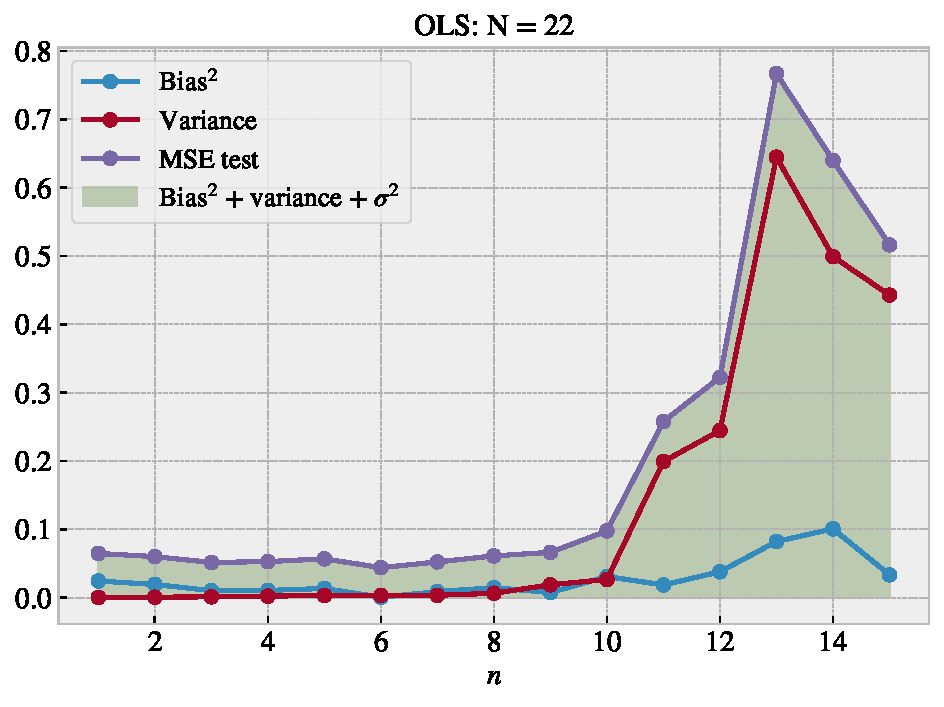
\includegraphics[width=0.8\linewidth]{figures/bias_variance_tradeoff_OLS.pdf}
    \caption{Bias-variance analysis for $N = 22$ and $\sigma = 0.2$ using the same number of bootstraps as traning points. We see that the main contribution to the test MSE comes from bias at low complexity and for variance at higher complexity.}
    \label{fig:bias_var_OLS}
\end{figure}
In figure \ref{fig:bias_var_OLS} we have investigated the tradeoff between high bias and low variance at low complexity vs low bias and high variance at high complexity. In our case the bias doesn't drop considerably for higher complexities when the variance increases (at $n \ge 10$). However, we see that the bias is the dominant error contributor at low complexities and variance is the dominant error contributor at higher complexities. Notice also that we get a perfect match with the theoretical decomposition done in section \ref{sec:bias_var_derivation} as the green coloring of figure \ref{fig:bias_var_OLS} confirms the relation
\begin{align*}
    \text{MSE} = \text{Bias}^2 + \text{variance} + \sigma^2.
\end{align*}
From figure \ref{fig:bias_var_OLS} we also observe that the MSE is at it lowest point for $n = 6$. \par
We now investigate the effect of varying the number of points, which turns out to affect the specific characteristics of the tradeoff quite a lot. The result is seen on figure \ref{fig:bias_var_OLS_multi}.
\begin{figure}[H]
    \centering
    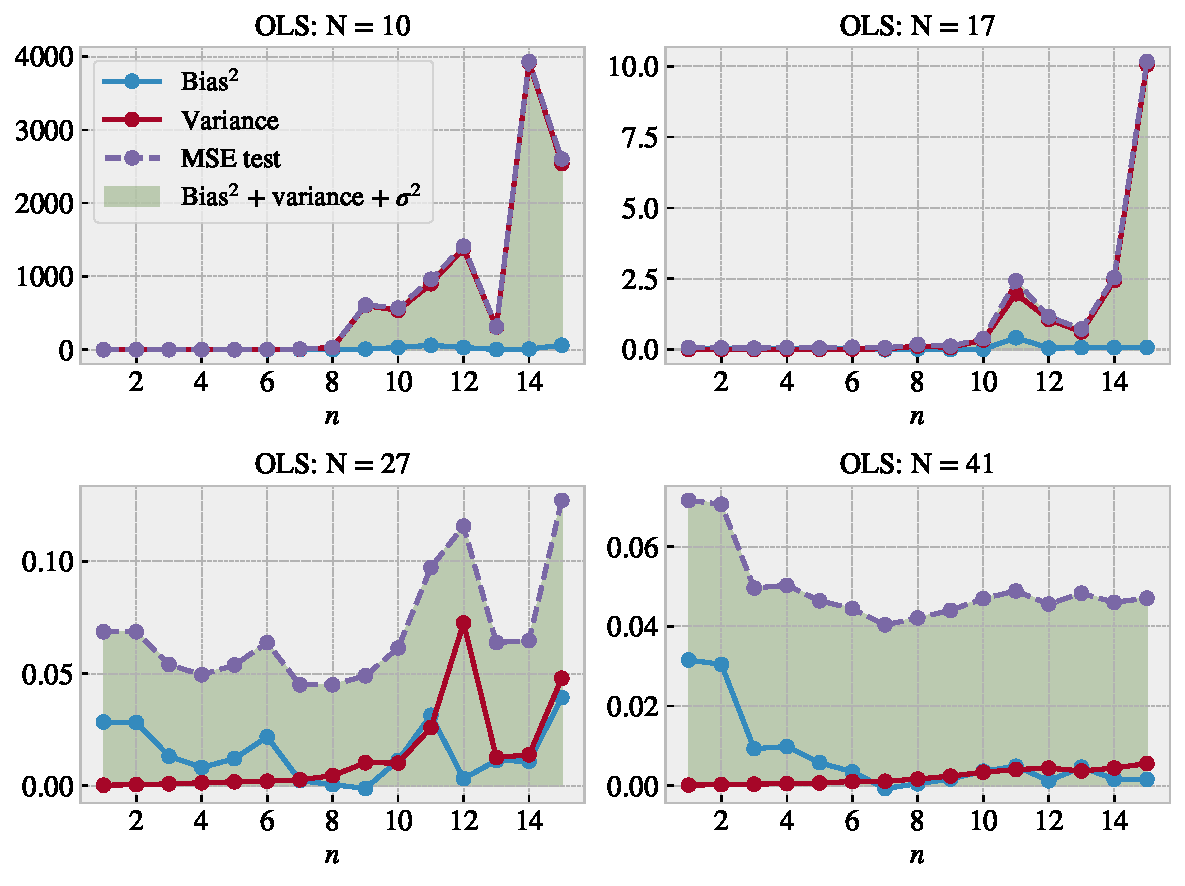
\includegraphics[width=\linewidth]{figures/bias_variance_tradeoff_OLS_2x2.pdf}
    \caption{Bias-variance analysis similar to figure \ref{fig:bias_var_OLS} but now with different choices of grid size: N = [10, 17, 27, 40].These was explicitly chosen to show some interesting features.}
     \label{fig:bias_var_OLS_multi}
\end{figure}

From \ref{fig:bias_var_OLS_multi} we see that the number of data points greatly affects the bias and variance relationship. Generally we see that that variance doesn't explode quite as drastically for higher $N$. This makes sense since the higher number of points makes the fitting less prone to overfitting. 

\section{Exercise 3}
In this exercise we will introduce the use of cross validation as a new resampling method for computing the MSE.

\subsection{Cross validation}
An alternative method to Bootstrap is Cross validation. Consider a dataset consisting of $m$ points. For a given value of k, cross validation splits the dataset into k parts. Then we label one part as test data and the rest as training data and compute the MSE. This is repeated k times by permuting the labels,  such that all parts are used as test data once (see figure \ref{fig:CV_example}). The total MSE is then calculated as a mean value of each k-fold. For some data sets it might be useful to shuffle the date before using cross validation in order to avoid having isolated trends of the data in only some folds. 

\begin{figure}[H]
    \centering
    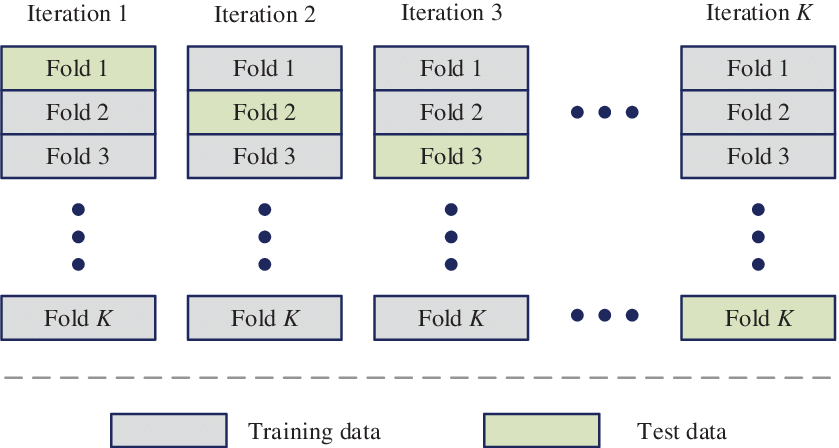
\includegraphics[width=0.70\textwidth]{figures/K-fold-cross-validation-method.png}
    \caption{K-fold cross validation example chart.}
    \label{fig:CV_example}
\end{figure}

To study the cross validation we perform OLS as a function of different complexity $n$ and compute the MSE using both cross validation and bootstrap. By varying the number of k-fold we compare these methods as shown in figure \ref{fig:CV_boot_comp}.

\begin{figure}[H]
     \centering
     \begin{subfigure}[b]{0.49\textwidth}
         \centering
         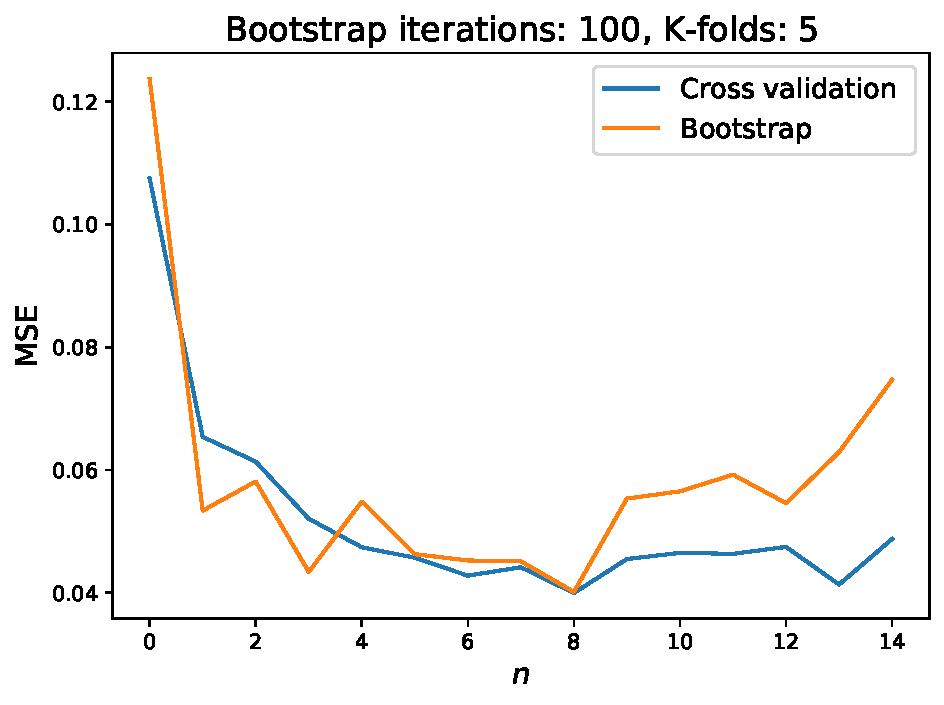
\includegraphics[width=\textwidth]{figures/CV_boot_comparison_with_k5.pdf}
         \caption{Cross validation and bootstrap comparison with k-fold number $=5$. }
         \label{fig:cv_b_5}
     \end{subfigure}
     \hfill
     \begin{subfigure}[b]{0.49\textwidth}
         \centering
         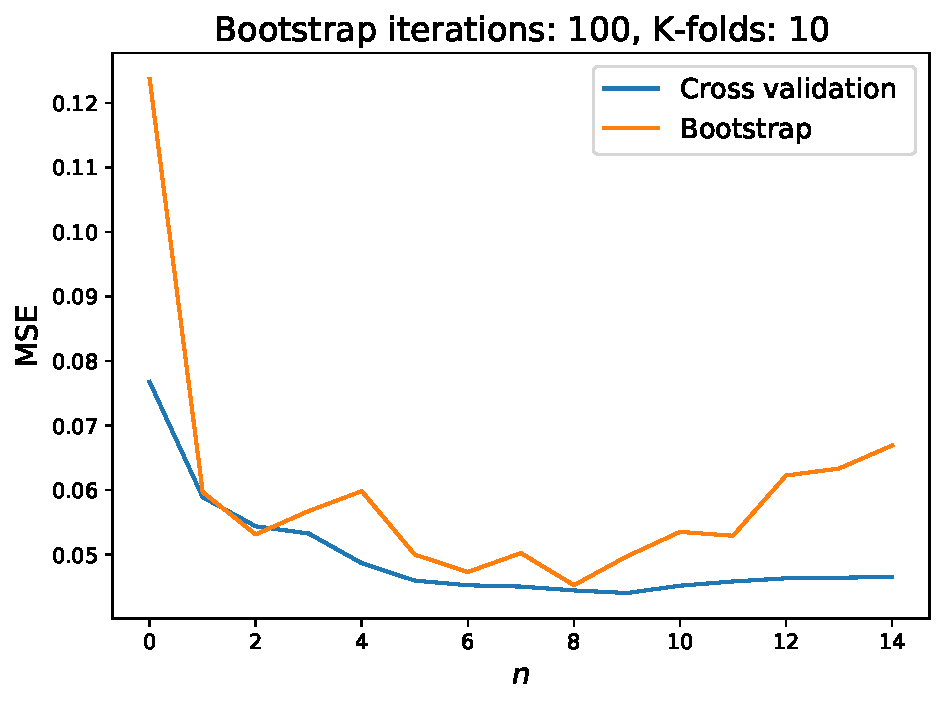
\includegraphics[width=\textwidth]{figures/CV_boot_comparison_with_k10.pdf}
         \caption{Cross validation and bootstrap comparison with k-fold number $=10$. }
         \label{fig:cv_b_10}
     \end{subfigure}
     \hfill
     \begin{subfigure}[b]{0.49\textwidth}
         \centering
         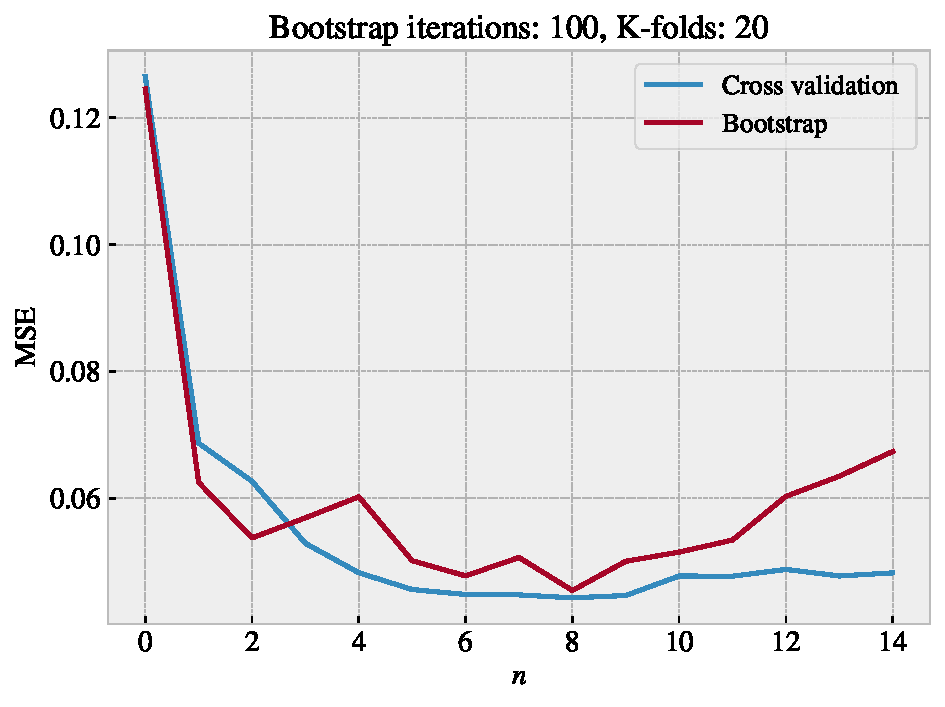
\includegraphics[width=\textwidth]{figures/CV_boot_comparison_with_k20.pdf}
         \caption{Cross validation and bootstrap comparison with k-fold number $=15$. }
         \label{fig:cv_b_20}
     \end{subfigure}
     \hfill
     \begin{subfigure}[b]{0.49\textwidth}
         \centering
         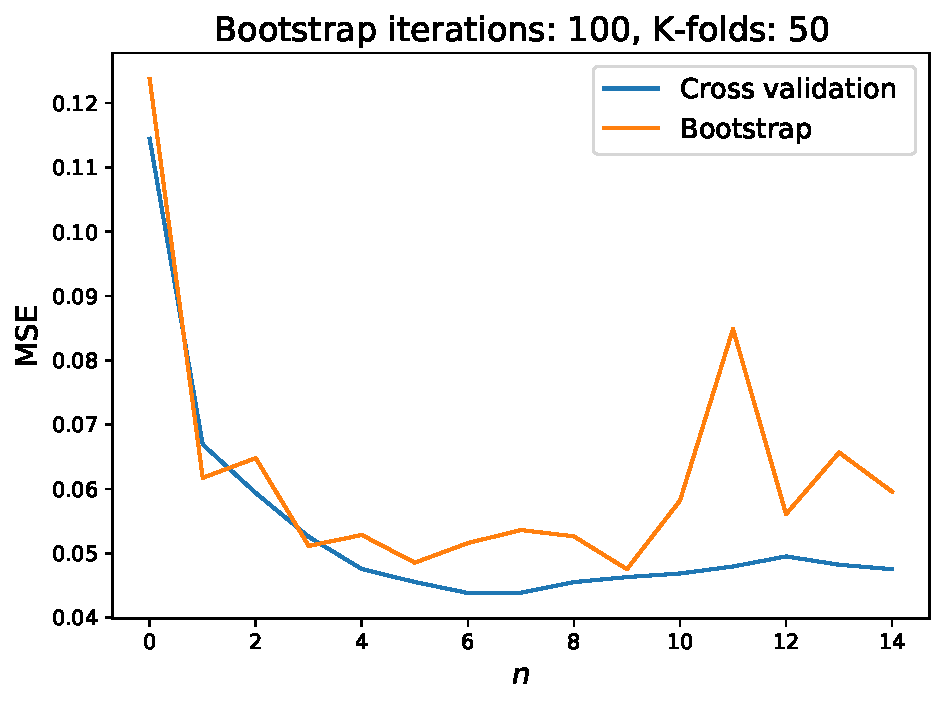
\includegraphics[width=\textwidth]{figures/CV_boot_comparison_with_k50.pdf}
         \caption{Cross validation and bootstrap comparison with k-fold number $=50$. }
         \label{fig:cv_b_50}
     \end{subfigure}
     
        \caption{OLS regression for varying complexity $n$. We compute  MSE by cross validation and bootstrap and compare for different numbers of k-fold. }
        \label{fig:CV_boot_comp}
\end{figure}

The ideal number of folds for a given situation is not easy to determine, as shown in figure \ref{fig:CV_boot_comp}. From the figure we observe that by increasing the number of k-folds, we get a more smooth trend for the cross validation MSE as a function of $n$. In general we see that the cross validation method yields lower MSE at higher complexities which is reinforced even more when k-folds is increased. When choosing the number of k-fold poorly we might get a misrepresentative evaluating of the model quality, which does not show from the results in figure \ref{fig:CV_boot_comp}. This can be either a model with high variance or high bias. For a final test of the model one could hold of some unseen test data to evaluate the model on. 
\\
% We would like to add that even though the MSE seems to not be heavily affected by the increase in number of folds, the method's ability to predict a data set is not necessarily equally effected. As the number of folds increases, so does the number of iterations. In addition, the size of the test data will decrease. For more iterations and smaller test data, it will be easier for the method to avoid over fitting and to predict that exact test data. But, by using a third set for validation, we believe that for a large number of folds, the method would predict poorly. Therefore, by choosing the number of k-fold poorly we might get a misrepresentative evaluating of the model quality, which does not show from the results in figure \ref{fig:CV_boot_comp}.

\section{Exercise 4}
In this exercise we introduce Ridge regression an repeat the bias-variance analysis and the MSE cross validation investigation. 
\subsection{Ridge Regression}
From section \ref{sec:exer1} we introduced an expression for the optimal $\beta$-values for OLS. The inverting of $\vec{X}^T\vec{X}$ yields no problem as long as the matrix is not singular. The Ridge method addresses this issue by introducing a parameter $\lambda$, such that the cost function becomes

\begin{align*}
    C(\vec{X}, \boldsymbol{\beta})=\frac{1}{n} \sum_{i=0}^{n-1}\left(z_{i}-\tilde{z}_i\right)^{2} + \frac{\lambda}{n} \sum_{i=0}^{n-1}\tilde{z}_i^2 =
    \frac{1}{n}\left[(\boldsymbol{z}-\boldsymbol{\tilde{z}})^{T}(\boldsymbol{z}-\boldsymbol{\tilde{z}}) + \lambda\boldsymbol{\tilde{z}}^2 \right], \qquad \vec{\tilde{z}} = \vec{X}\boldsymbol{\beta},
\end{align*}
which gives us the optimal $\beta$ as 
\begin{align*}
    \hat{\boldsymbol{\beta}} = (\vec{X}^T\vec{X} + \lambda \boldsymbol{I} )^{-1}\vec{X}^T\vec{z}.
\end{align*}



\newpage
\subsection{Ridge analysis }


Firstly we repeat the comparison of bootstrap and cross validation using the Ridge regression method. However, this time we will do the comparison for varying values of $\lambda$. The result is shown in figure \ref{fig:CV_B_Ridge}.
\begin{figure}[H]
     \centering
     \begin{subfigure}[b]{0.49\textwidth}
         \centering
         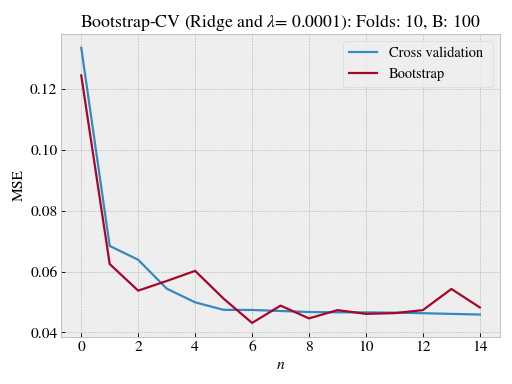
\includegraphics[width=\textwidth]{figures/CV_B_Ridge_0001.png}
         \caption{Bootstrap, cross validation comparison for Ridge with $\lambda = \num{1e-4}$.}
        \label{fig:CV_B_Ridge0001}
     \end{subfigure}
    \hfill
     \begin{subfigure}[b]{0.49\textwidth}
         \centering
         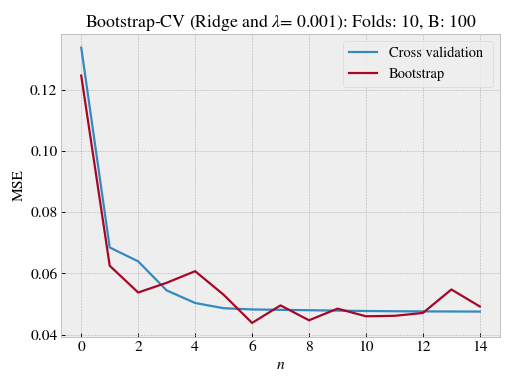
\includegraphics[width=\textwidth]{figures/CV_B_Ridge_001.png}
        \caption{Bootstrap, cross validation comparison for Ridge with $\lambda = \num{1e-3}$.}
    \label{fig:CV_B_Ridge001}
     \end{subfigure}
    \begin{subfigure}[b]{0.49\textwidth}
         \centering
         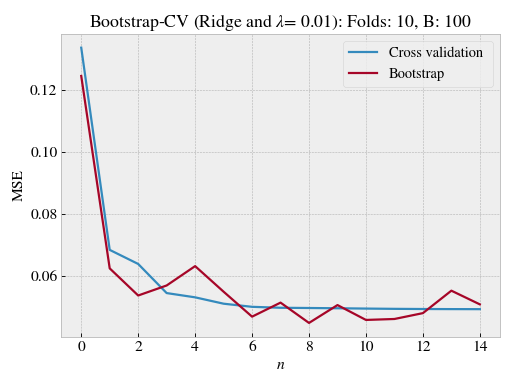
\includegraphics[width=\textwidth]{figures/CV_B_Ridge_01.png}
          \caption{Bootstrap, cross validation comparison for Ridge with $\lambda = \num{1e-2}$.}
          \label{fig:CV_B_Ridge01}
     \end{subfigure}
     \hfill
     \begin{subfigure}[b]{0.49\textwidth}
         \centering
         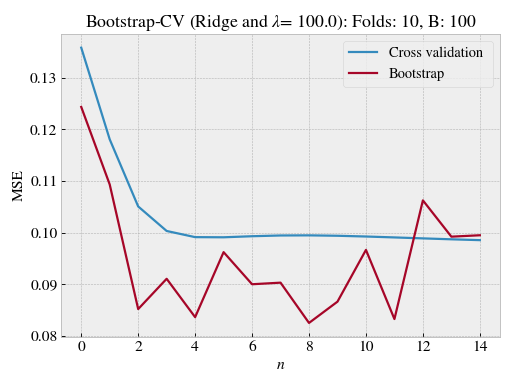
\includegraphics[width=\textwidth]{figures/CV_B_Ridge_100.png}
         \caption{Bootstrap, cross validation comparison for Ridge with $\lambda = \num{1e2}$.   }
        \label{fig:fig:CV_B_Ridge1}
     \end{subfigure}
    \caption{Bootstrap, cross validation comparison for Ridge method with N = 30, $\sigma = 0.2$, 10 folds, 100 bootstraps and varying values for $\lambda$.}
    \label{fig:CV_B_Ridge}
\end{figure}
From figure \ref{fig:CV_B_Ridge} we observe that both bootstrap and cross validation gives relatively similar MSE-values for lower values of $\lambda$ (figures \ref{fig:CV_B_Ridge0001} through \ref{fig:CV_B_Ridge01}). When increasing $\lambda$ to 100, bootstrap yields lower MSE values then cross validation.\par 
Next we repeat the bias-variance analysis using Ridge regression as shown in figure \ref{fig:b_v_ridge}.

\begin{figure}[H]
     \centering
     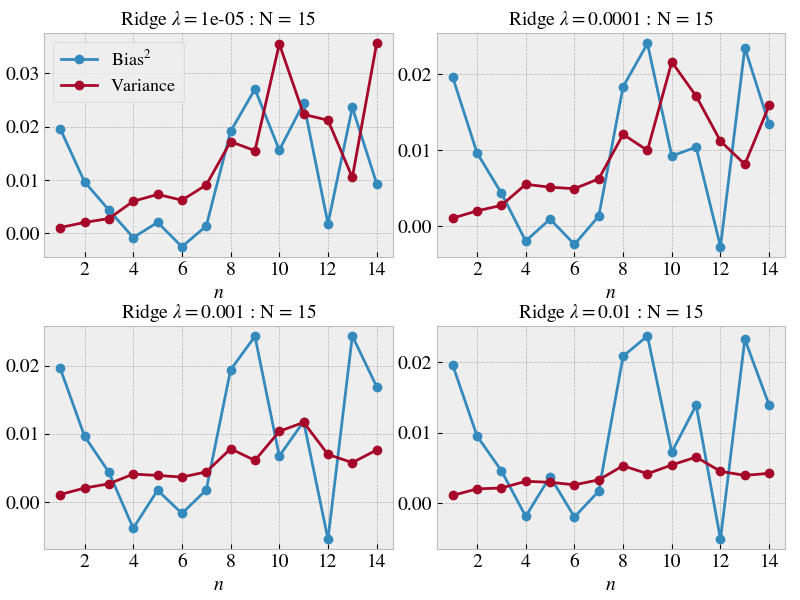
\includegraphics[width=\textwidth]{figures/BVT_Ridge.png}
     \caption{Bias variance trade-off for Ridge-method with $\lambda$-values [1e-5,1e-4,1e-3,1e-2], N =15 and $B = 100$.}
     \label{fig:b_v_ridge}
\end{figure}
In figure \ref{fig:b_v_ridge} we have calculated the bias and  variance for N = 15 and 100 bootstraps using the Ridge method. For small $\lambda$ we see a trend that is somewhat similar to the bias-variance analysis done for OLS. This is expected as Ridge approximates OLS when $\lambda$ is small. For larger values of $\lambda$ the variance decreases and the bias starts to dominate the error. Thus the introduction of $\lambda$ effectively dampens the variance. Thus it can be interesting to study the evolution of $\beta$-values as $\lambda$ is increased.
\newline

In figure \ref{fig:lamda_depend} we study the values of $\beta$ as a function of $\lambda$. The figure shows that as $\lambda$ increases, the absolute values of beta is forced towards 0. Hence the variance of the $\beta$'s decrease, and this supports the finding from figure \ref{fig:CV_B_Ridge}  that increasing $\lambda$ decreases the variance in the Ridge regression. This, together with the findings from \ref{fig:CV_B_Ridge}, shows that bootstrap handles the error from the bias better than cross validation when using Ridge.
\begin{figure}[H]
    \centering
    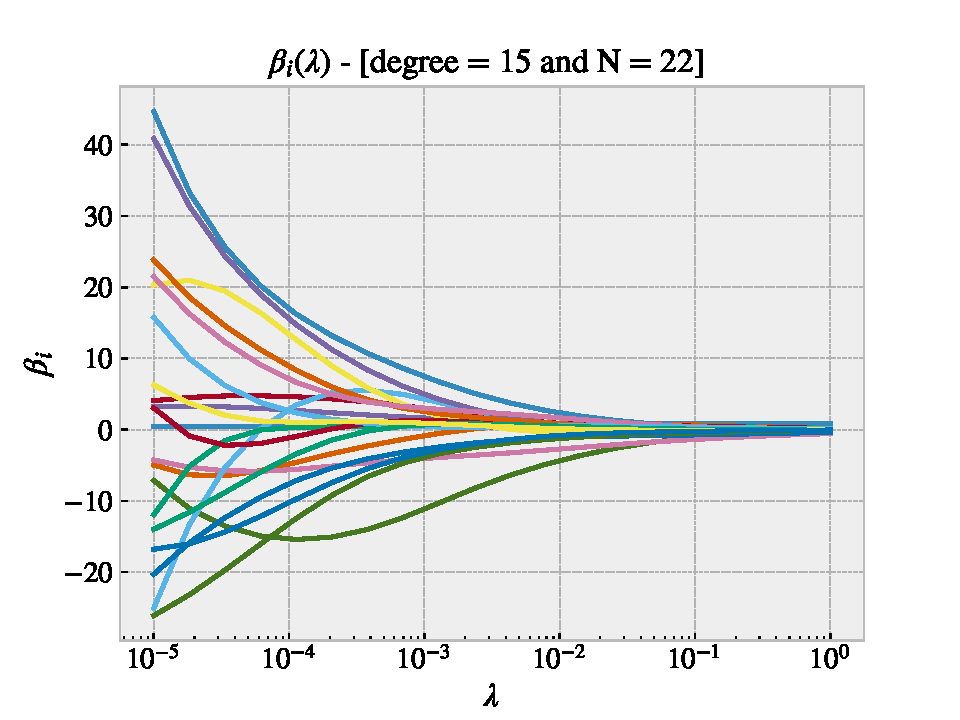
\includegraphics[width=0.80\textwidth]{figures/lamda_depend_betas.pdf}
    \caption{$\beta_i$ as a function of $\lambda$ for $N = 15$ and $n = 15$.}
    \label{fig:lamda_depend}
\end{figure}
Note also that some of the bias$^2$-values in figure (\ref{fig:b_v_ridge}) are negative, which should not be possible. This can be explained by the fact that we based our calculation on the assumption that the noise is drawn from a normal distribution such that the mean value is 0 and the variance $\sigma^2$. When sampling the noise numerically, for a limited number of points, the calculation of bias as 
\begin{align*}
    \text{bias}^2 = \E[(y  -\E[\Tilde{y}])^2] - \sigma^2,
\end{align*}
does not nessecary hold true. 
\newpage

\section{Exercise 5}
In this exercise we introduce Lasso regression and repeat the bias-variance analysis and the MSE cross validation investigation.

\subsection{Lasso Regression}
Another regression method is Lasso regression. For this method we define the cost function by taking the absolute value of beta instead of the square, giving us 

\begin{align*}
    C(\vec{X}, \boldsymbol{\beta})=\frac{1}{n} \sum_{i=0}^{n-1}\left(z_{i}-\tilde{z}_i\right)^{2} + \frac{\lambda}{n} \sum_{i=0}^{n-1}\mid \tilde{z}_i \mid =
    \frac{1}{n}\left[(\boldsymbol{z}-\boldsymbol{\tilde{z}})^{T}(\boldsymbol{z}-\boldsymbol{\tilde{z}}) + \lambda\mid \boldsymbol{\tilde{z}}\mid \right], \qquad \vec{\tilde{z}} = \vec{X}\boldsymbol{\beta}.
\end{align*}


\subsection{Lasso analysis}
As we did for Ridge, we will do a comparison between bootstrap and cross validation. The result is shown in figure \ref{fig:CV_B_Lasso}.
\begin{figure}[H]
     \centering
     \begin{subfigure}[b]{0.49\textwidth}
         \centering
         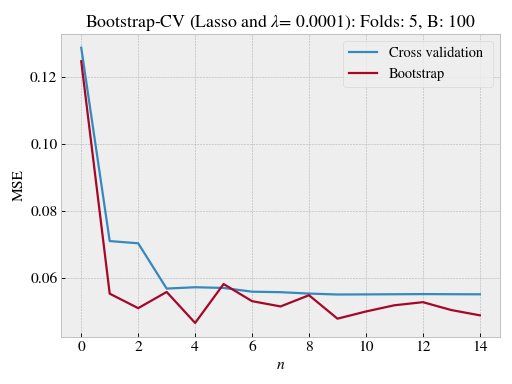
\includegraphics[width=\textwidth]{figures/CV_B_Lasso_0001.png}
         \caption{Bootstrap, cross validation comparison for Lasso with $\lambda = \num{1e-4}$.}
        \label{fig:CV_B_Lasso0001}
     \end{subfigure}
    \hfill
     \begin{subfigure}[b]{0.49\textwidth}
         \centering
         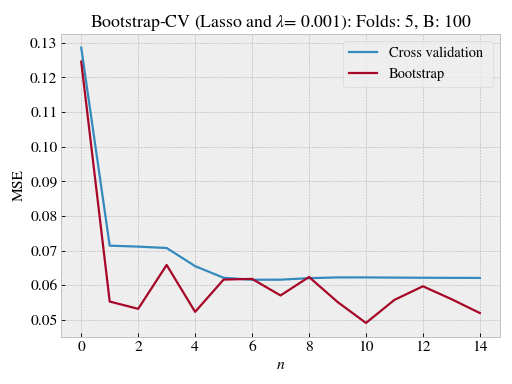
\includegraphics[width=\textwidth]{figures/CV_B_Lasso_001.png}
        \caption{Bootstrap, cross validation comparison for Lasso with $\lambda = \num{1e-3}$.}
    \label{fig:CV_B_Lasso001}
     \end{subfigure}
    \begin{subfigure}[b]{0.49\textwidth}
         \centering
         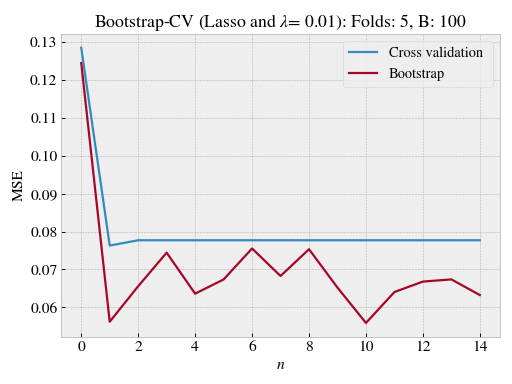
\includegraphics[width=\textwidth]{figures/CV_B_Lasso_01.png}
          \caption{Bootstrap, cross validation comparison for Lasso with $\lambda = \num{1e-2}$.}
          \label{fig:CV_B_Lasso1}
     \end{subfigure}
     \hfill
     \begin{subfigure}[b]{0.49\textwidth}
         \centering
         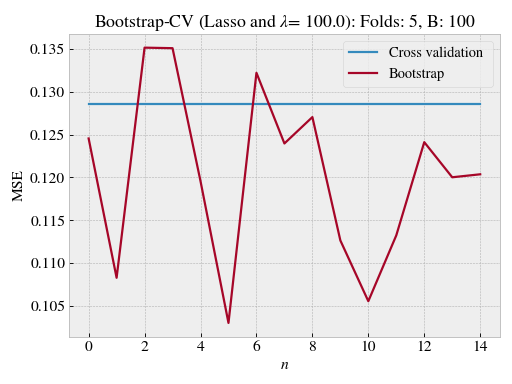
\includegraphics[width=\textwidth]{figures/CV_B_Lasso_100.png}
         \caption{Bootstrap, cross validation comparison for Lasso with $\lambda = \num{1e2}$.   }
        \label{fig:fig:CV_B_Lasso1}
     \end{subfigure}
    \caption{Bootstrap, cross validation comparison for Lasso method with N = 30, $\sigma = 0.2$, 10 folds, 100 bootstraps and varying values for $\lambda$.}
    \label{fig:CV_B_Lasso}
\end{figure}
In figure \ref{fig:CV_B_Lasso} we observe a somewhat similar trend as in figure \ref{fig:CV_B_Ridge} for small values (figure \ref{fig:CV_B_Lasso0001} and \ref{fig:CV_B_Lasso001}) of $\lambda$. when using Ridge, we observed that the trend for cross validation MSE gradually "flattens out" when increasing $\lambda$. In the case of Lasso regression the cross validation MSE "flattens out" completely.
\\
In figure \ref{fig:B_T_lasso} we have study again the Bias-variance trade-off with the Lasso method.  Similar to the case of Ridge regression we see that an increased $\lambda$ result in a dampening of the variance. However, we see that the dampening is stronger for the Lasso method compared to Ridge given the same $\lambda$-parameter. We also find cases of negative bias$^2$ values for this result, for which the same explanation as used earlier, holds.

\begin{figure}[H]
    \centering
    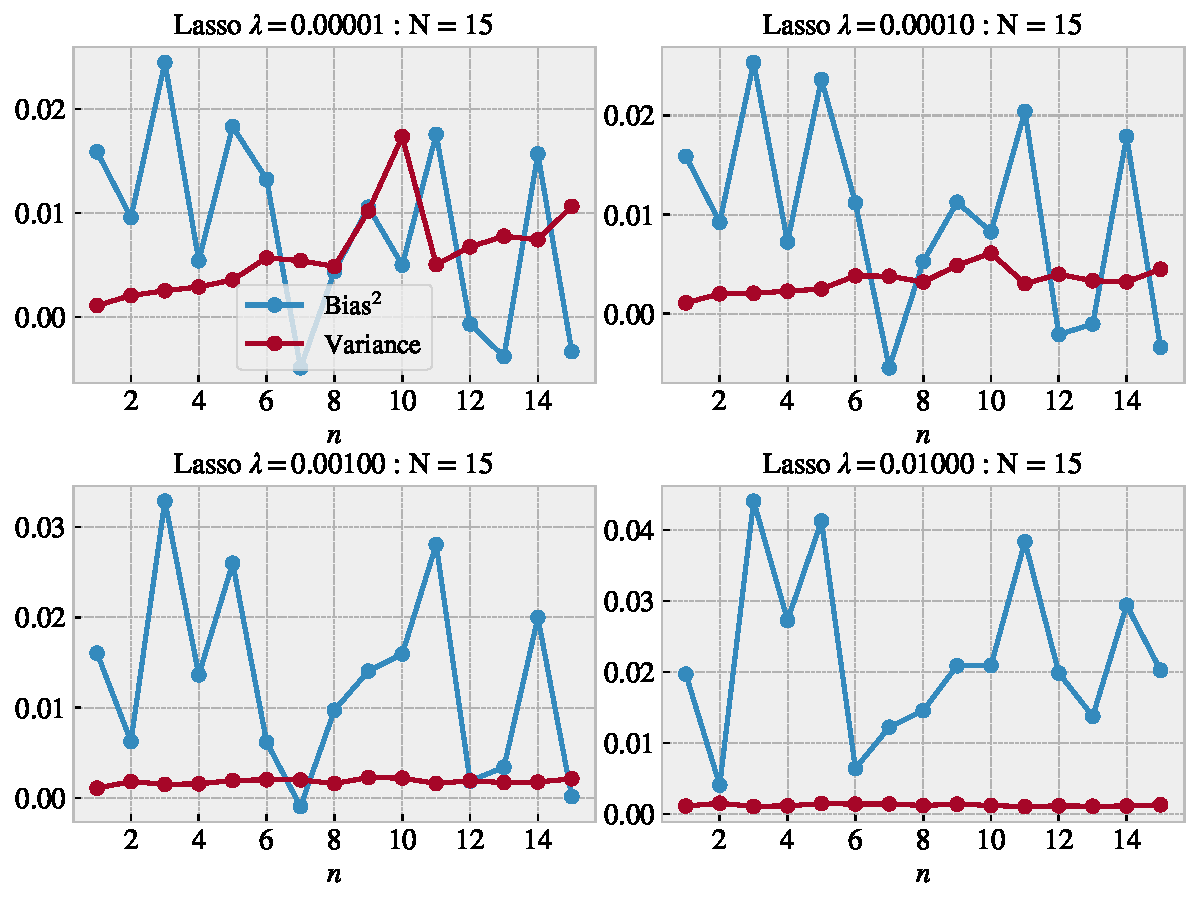
\includegraphics[width=0.70\textwidth]{figures/bias_variance_tradeoff_Lasso_2x2.pdf}
    \caption{ Bias Variance trade-off for Lasso with $N=15$ and varying $\lambda \in [10^{-5}, 10^{-1}]$}
    \label{fig:B_T_lasso}
\end{figure}



\subsection{Finding the best model for Franke's function}\label{sec:franke_model}
We will now investigate which regression fits the general trend of Franke's function the best. We begin by estimating the best hyperparameters for each regression method: OLS, Ridge, and Lasso respectively. We generate a data set with $N = 30$ and noise $\sigma = 0.2$, and use the usual 80-20\% split. We then perform regression on the training set and evaluate the MSE by cross validation (with 5 k-folds) for different combinations of hyperparameters $n$ and $\lambda$. The result is shown for OLS in figure \ref{fig:OLS_franke_hyper}, for Ridge in figure \ref{fig:Ridge_franke_hyper} and Lasso in figure \ref{fig:Lasso_franke_hyper}.

\begin{figure}[H]
    \centering
    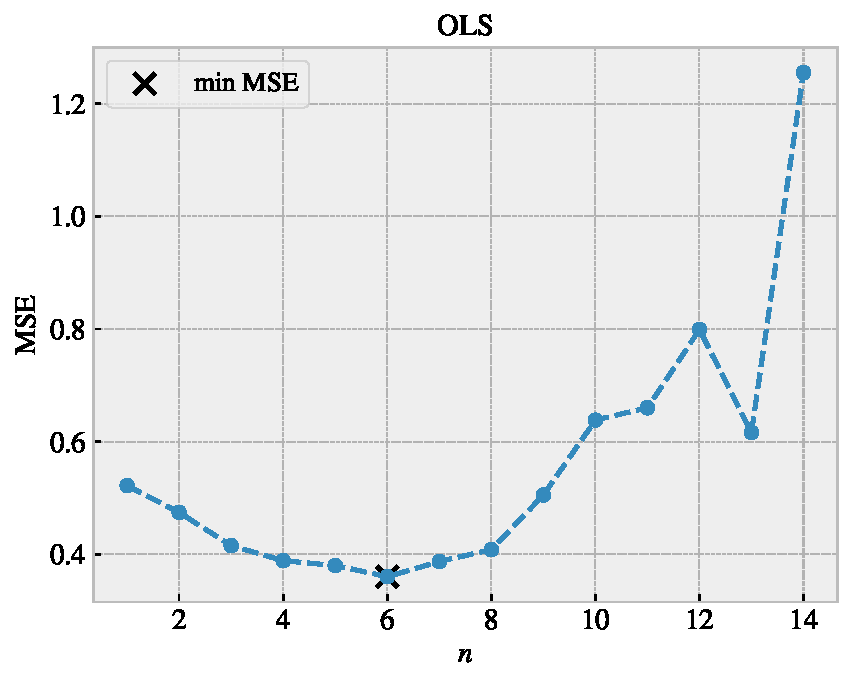
\includegraphics[width=0.60\textwidth]{figures/Franke_best_OLS_map_B.pdf}
    \caption{ Estimation of best hyperparameter for OLS on Franke's function. The plot shows MSE  (found  by  k-fold  =  5  cross  validation)  for  the  training  data  with varying n. The minimum MSE error is achieved for n=6.}
    \label{fig:OLS_franke_hyper}
\end{figure}

\begin{figure}[H]
    \centering
    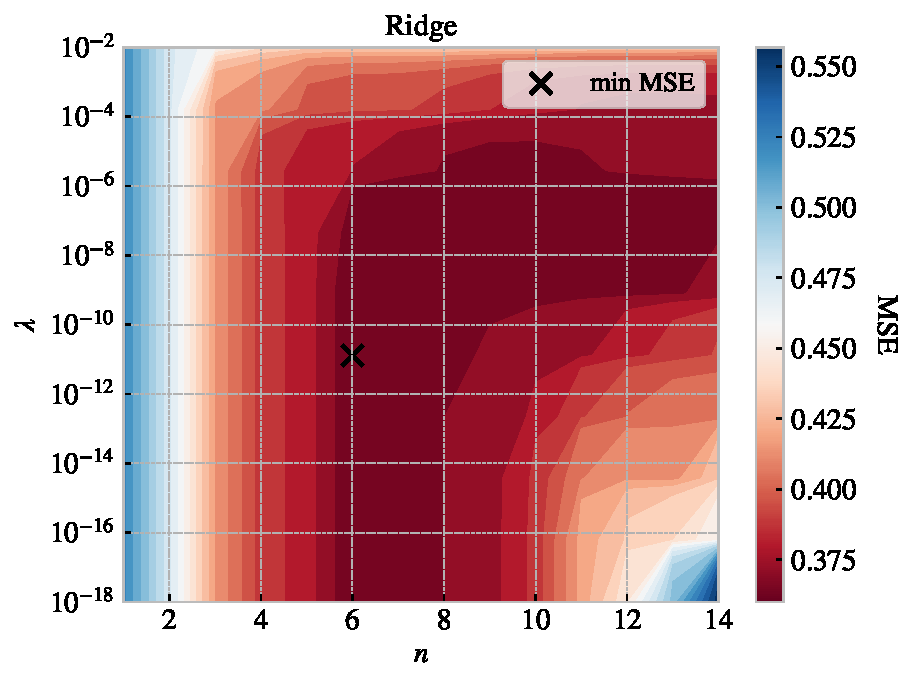
\includegraphics[width=0.7\textwidth]{figures/Franke_best_Ridge_map_B.pdf}
    \caption{Estimation of best hyperparameter for Ridge on Franke's function. The plot shows MSE (found by k-fold = 5 cross validation) for the training data with varying $n$ and $\lambda$. The minimum MSE error is achieved for $n = 6$, $\lambda = \num{1.3e-11}$.}
    \label{fig:Ridge_franke_hyper}
\end{figure}

\begin{figure}[H]
    \centering
    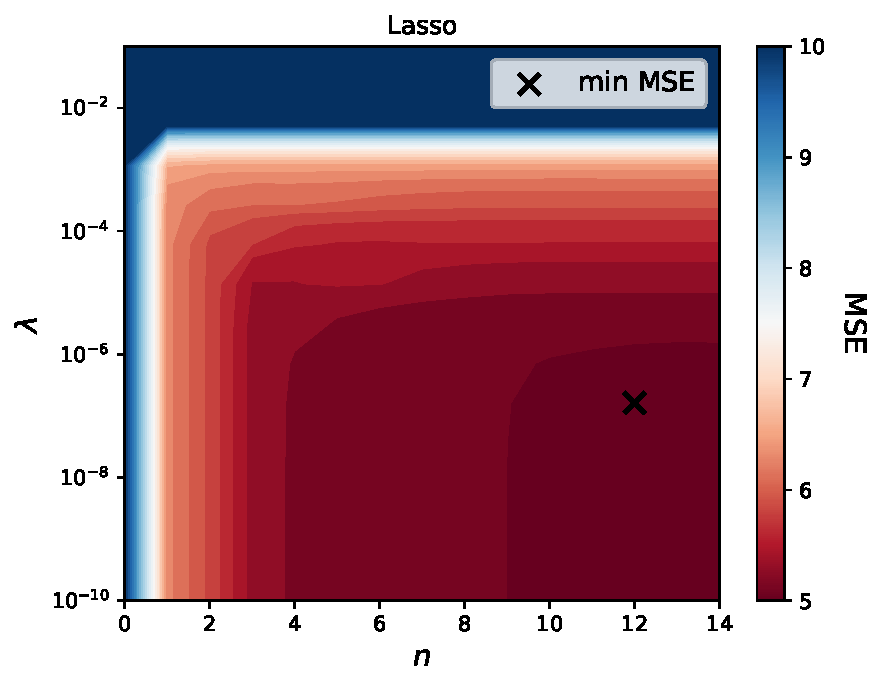
\includegraphics[width=0.7\textwidth]{figures/Franke_best_Lasso_map_B.pdf}
    \caption{Estimation of best hyperparameter for Lasso on terrain data. The plot shows MSE (found by k-fold = 5 cross validation) for the training data with varying $n$ and $\lambda$. The minimum MSE error is achieved for $n = 13$, $\lambda = \num{2.8e-6}$. }
    \label{fig:Lasso_franke_hyper}
\end{figure}

\newbreak
From figure \ref{fig:OLS_franke_hyper}, \ref{fig:Ridge_franke_hyper}  \ref{fig:Lasso_franke_hyper} we find the best hyperparameters to be as shown in table \ref{tab:Franke_hyper}.

\begin{table}[H]
  \begin{center}
  \caption{The best hyperparameters for OLS, Ridge and Lasso regression on Franke's function found from figure \ref{fig:OLS_franke_hyper}, \ref{fig:Ridge_franke_hyper} and \ref{fig:Lasso_franke_hyper}.}
  \begin{tabular}{|c|c|c|c|} \hline
    & \text{OLS} & \text{Ridge} & \text{Lasso}  \\\hline
    $n$ & 6 & 6 & 13   \\\hline
    $\lambda$ &  NA &  \num{1.3e-11}  & \num{2.8e-6}  \\\hline
  \end{tabular}
  \label{tab:Franke_hyper}
  \end{center}
\end{table}

Using the optimal hyperparameters for each regression method we compute the predictions on the test data and evaluate the MSE between the predictions and the test data target points. On figure \ref{fig:test_data_3D} we have shown the test data which we aim to replicate by the model predictions, as shown in figure \ref{fig:franke_hyper_pred}.


\begin{figure}[H]
     \centering
     \begin{subfigure}[b]{0.49\textwidth}
         \centering
         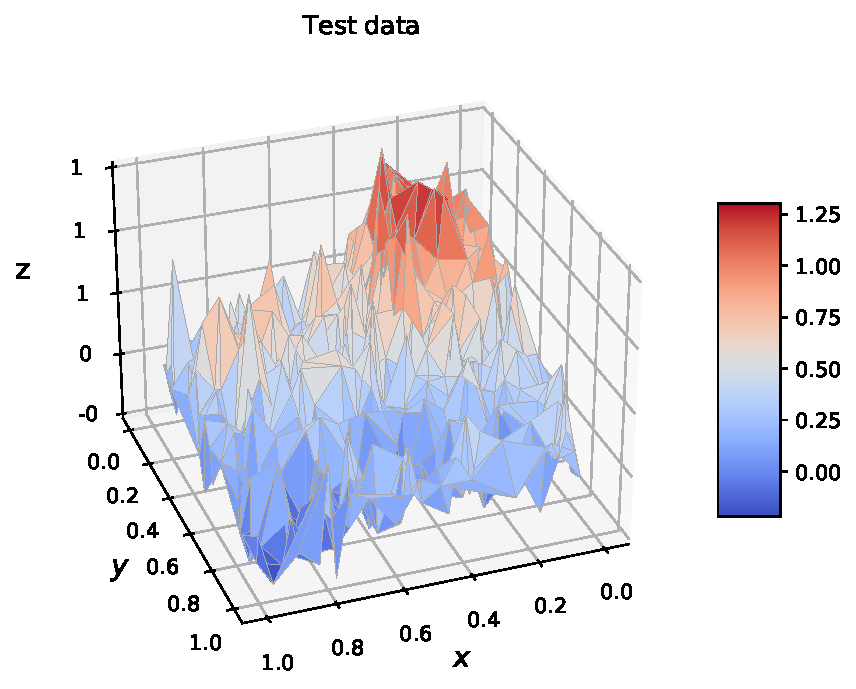
\includegraphics[width=\textwidth]{figures/Franke_test_data.pdf}
         \caption{Test data from Franke's function for N = 30 and $\sigma = 0.2$ }
        \label{fig:test_data_3D}
     \end{subfigure}
    \hfill
     \begin{subfigure}[b]{0.49\textwidth}
         \centering
         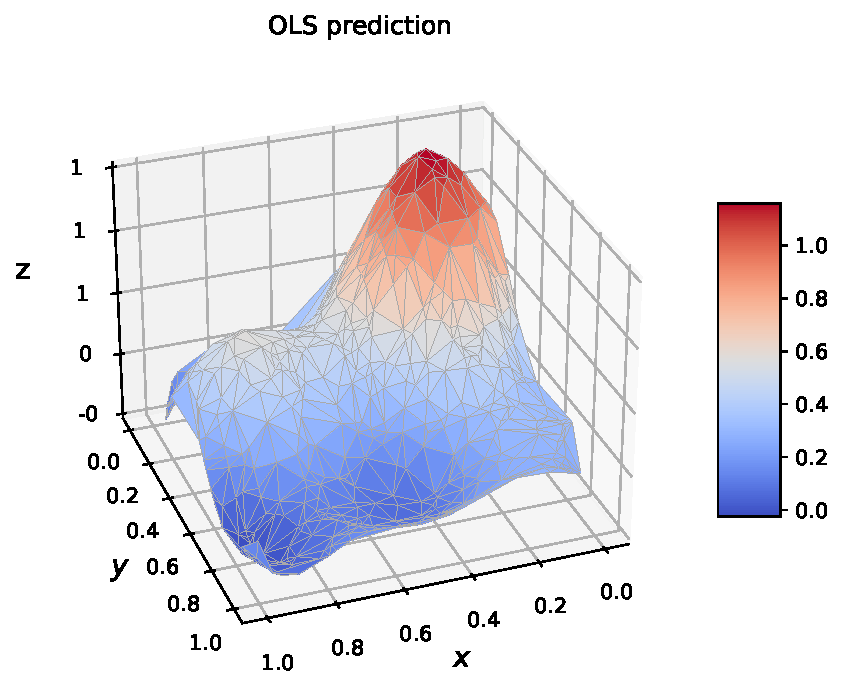
\includegraphics[width=\textwidth]{figures/Franke_OLS_predict.pdf}
        \caption{Predictions of the test data for OLS method with n = 6.}
    \label{fig:OLS_test_predict}
     \end{subfigure}
    \begin{subfigure}[b]{0.49\textwidth}
         \centering
         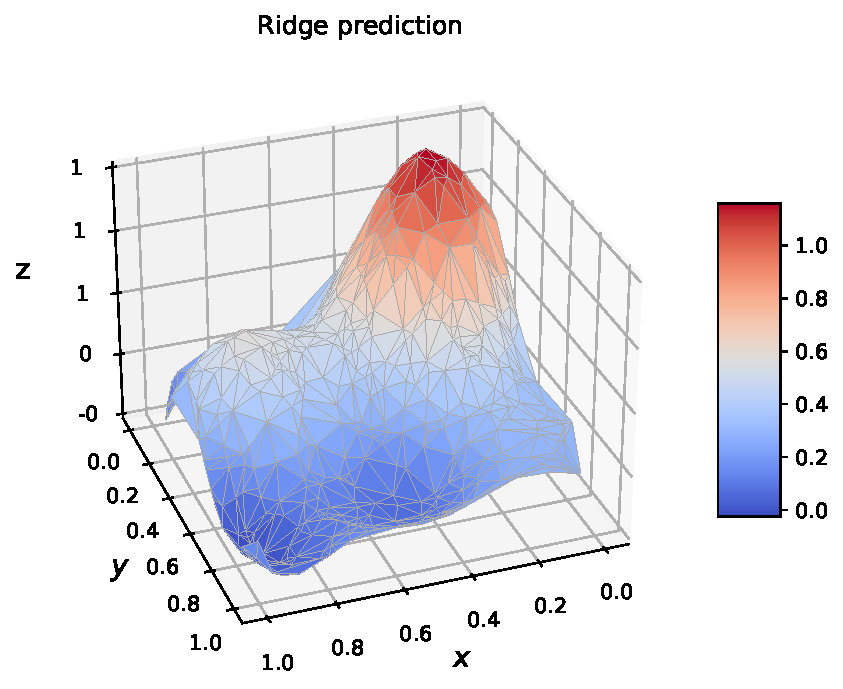
\includegraphics[width=\textwidth]{figures/Franke_Ridge_predict.pdf}
          \caption{Predictions of the test data for Ridge method with n = 6 and $\lambda =  \num{1.3e-11}$. }
          \label{fig:Ridge_test_predict}
     \end{subfigure}
     \hfill
     \begin{subfigure}[b]{0.49\textwidth}
         \centering
         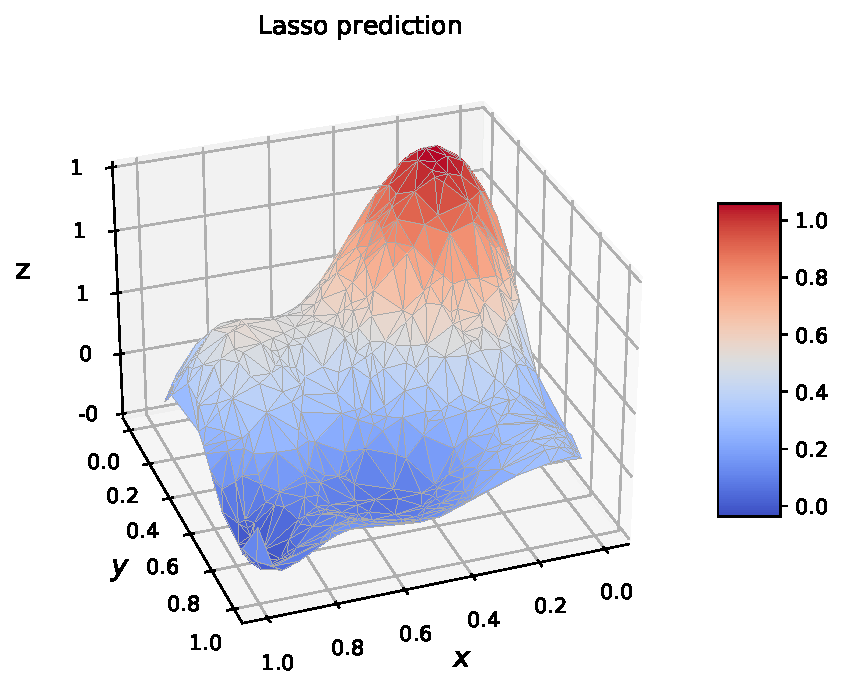
\includegraphics[width=\textwidth]{figures/Franke_Lasso_predict.pdf}
         \caption{Predictions of the test data for Lasso method with n = 13 and $\lambda =\num{2.8e-6}$.   }
        \label{fig:Lasso_test_predict}
     \end{subfigure}
    \caption{Comparing the predictions Subfigure}
    \label{fig:franke_hyper_pred}
\end{figure}


From figure \ref{fig:franke_hyper_pred} we see that all three methods create prediction that resemble the Franke function quite well (see figure \ref{fig:z_func}). This confirms visually that all three methods were able to find the general trend of the Franke function even with the added noise. We confirm this by computing the MSE between the predictions and the test data as shown in table \ref{tab:MSE_all_methods}.
\begin{table}[H]
  \begin{center}
  \caption{MSE score between the predictions and the test data with methods; OLS, Ridge and Lasso, using the optimal hyperparameters found from extensively training.}
  \begin{tabular}{|c|c|c|c|} \hline
  & \text{OLS} & \text{Ridge} & \text{Lasso} \\
  \hline
  \text{MSE} & 0.33894 & 0.33894 & 0.34050  \\ 
  \hline
  \end{tabular}
  \label{tab:MSE_all_methods}
  \end{center}
\end{table}
From table \ref{tab:MSE_all_methods} we see that the predictions yields relatively small MSE on a similar order of magnitude. For this exact run we got a equal MSE for both OLS and Ridge, which was slightly lower then the error for Lasso.  We notice that the optimal $\lambda$-value for Ridge is very small (magnitude of $10^{-11}$), for which the method effectively approaches OLS as $\lambda \rightarrow 0$. Therefore a conclusion to this specific settings is that OLS fits the data well. \\
However, this is not to be taken as an absolute fact as the computation of the best hyperparemeters for Ridge and Lasso was flawed by computational inadequacy. When searching for low $\lambda$-values the converging of the Ridge and Lasso regressions required a high number of iterations. This came across as a convergence error in the Sklearn package. When respecting the need for extra iterations we had to run with a number of max iterations $>10^6$ for which it became computationally heavy to find a minimum MSE in the hyperparameter search. Thus our best change of finding a minimum was to use $\num{1e4}$ as the maximum number of interations and thus ignoring the warning. Therefore we must treat or results as a comparison between the methods. Thus the determined optimal hyperparameters for each method might not be as accurate.
\newpage

\section{Exercise 6}

\subsection{Test models on Terrain}
In this exercise we will use OLS, Ridge, and Lasso regression respectively to analyze real terrain data. By using the website \url{https://earthexplorer.usgs.gov/} we are able to retrieve real world terrain data. We choose a hilly area in Saudi Arabia which is shown in figure \ref{fig:terrain_data}. The original resolution was quite high, so in order to process the data faster we reduced it to $37 \times 37$ (1369) data points. Due to lack of information regarding the units we treat them simply as unknown length units.
\\
\begin{figure}[H]
    \centering
    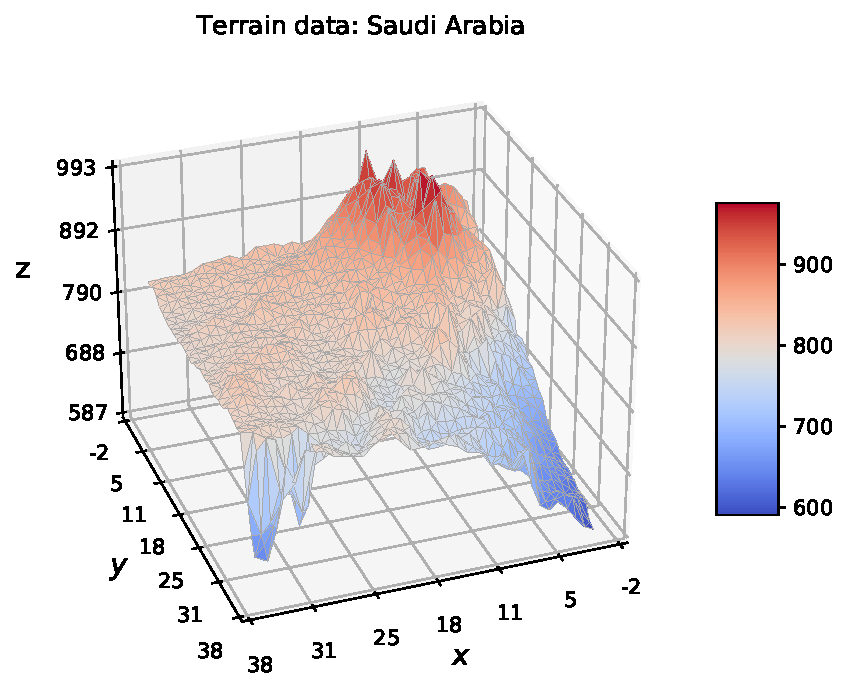
\includegraphics[width=0.8\textwidth]{figures/terrain_data.pdf}
    \caption{Terrain data from Saudi Arabia with $N \times N = 37 \times 37$ (1369 data points). We treat the units as unknown length units.}
    \label{fig:terrain_data}
\end{figure}
We perform a similar investigation on the terrain data as done in exercise 5 to determine the best hyperparameters for each regression method and then compare the MSE on the test data. The search for the best hyperparameters is shown in figure \ref{fig:OLS_terrain_hyper}, \ref{fig:Ridge_terrain_hyper} and \ref{fig:Lasso_terrain_hyper}.

\begin{figure}[H]
    \centering
    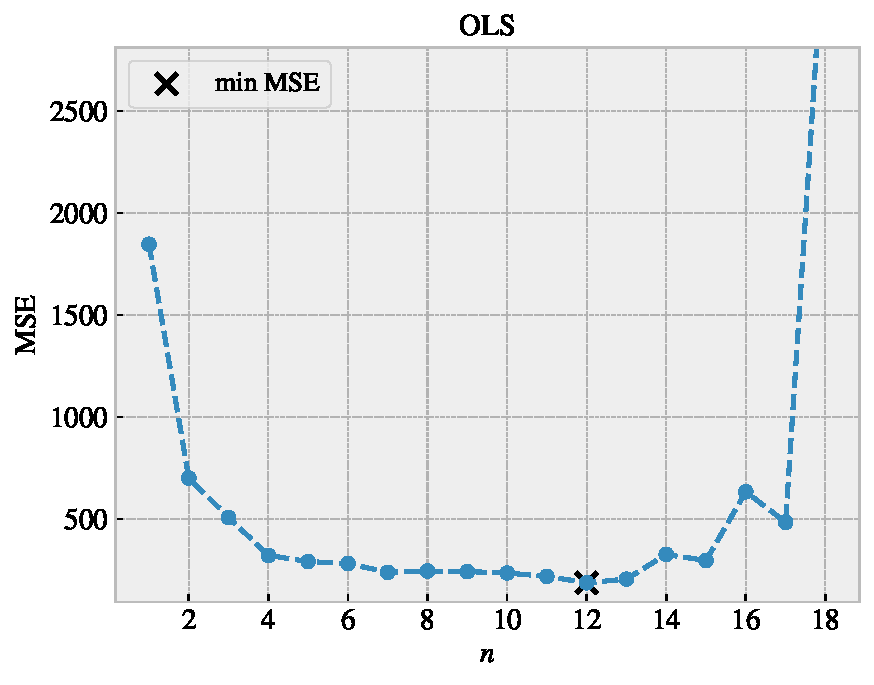
\includegraphics[width=0.7\textwidth]{figures/real_data_best_OLS_map_BM.pdf}
    \caption{Estimation of best hyperparameter for OLS on terrain data. The plot shows MSE (found by k-fold = 5 cross validation) for the training data with varying$ n$. The minimum MSE error is achieved for $n = 11$. }
    \label{fig:OLS_terrain_hyper}
\end{figure}

\begin{figure}[H]
    \centering
    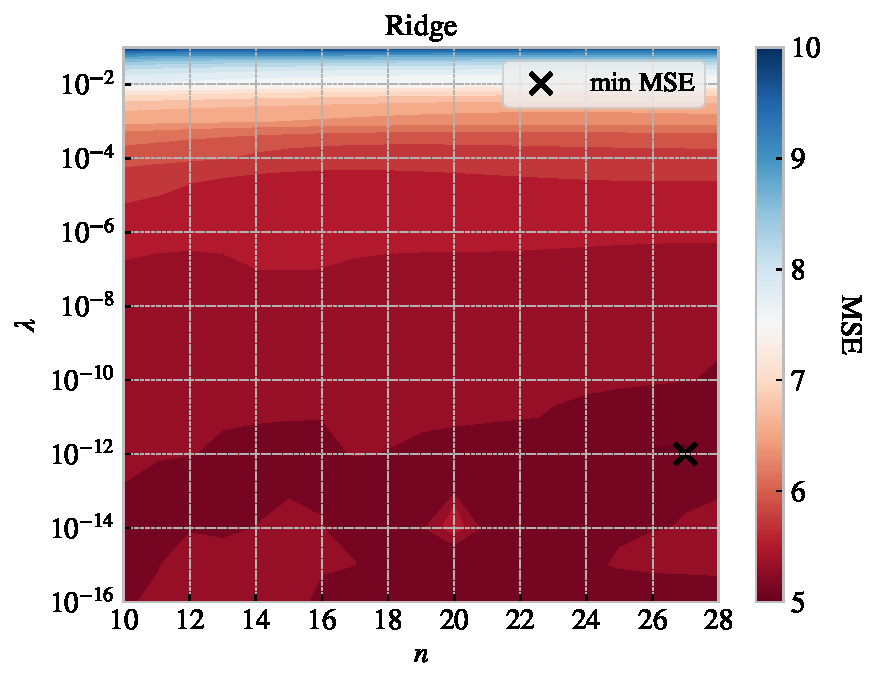
\includegraphics[width=0.7\textwidth]{figures/real_data_best_Ridge_map_BM.pdf}
    \caption{Estimation of best hyperparameter for Ridge on terrain data. The plot shows MSE (found by k-fold = 5 cross validation) for the training data with varying $n$ and $\lambda$. The minimum MSE error is achieved for $n = 12$, $\lambda = \num{2.7e-10}$.}
    \label{fig:Ridge_terrain_hyper}
\end{figure}

\begin{figure}[H]
    \centering
    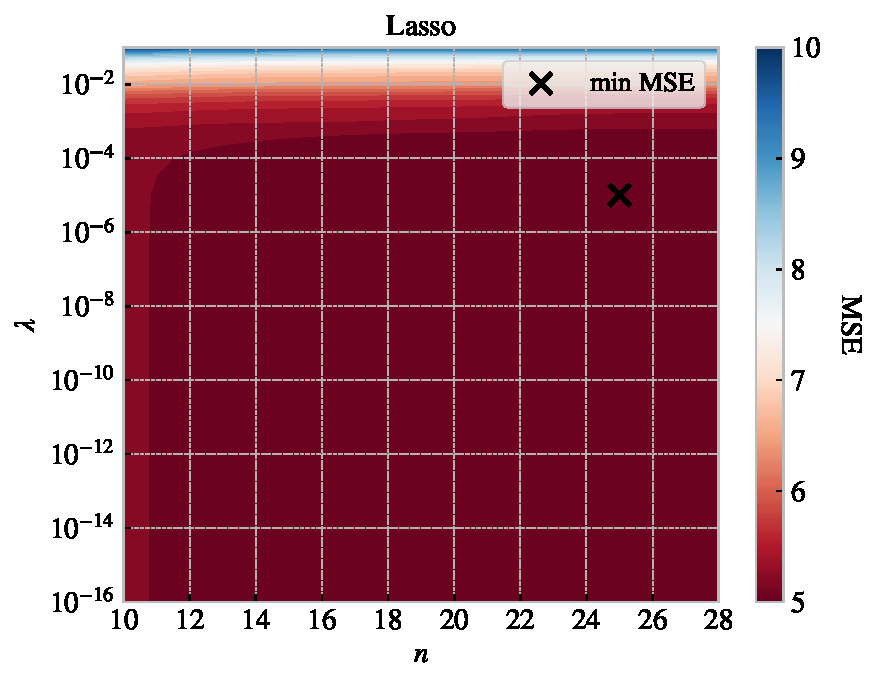
\includegraphics[width=0.7\textwidth]{figures/real_data_best_Lasso_map_BM.pdf}
    \caption{Estimation of best hyperparameter for Lasso on terrain data. The plot shows MSE (found by k-fold = 5 cross validation) for the training data with varying $n$ and $\lambda$. The minimum MSE error is achieved for $n = 19$, $\lambda = \num{4.4e-7}$.}
    \label{fig:Lasso_terrain_hyper}
\end{figure}

From figure \ref{fig:OLS_terrain_hyper}, \ref{fig:Ridge_terrain_hyper}  \ref{fig:Lasso_terrain_hyper} we find the best hyperparameters to be as shown in table \ref{tab:Franke_hyper}.

\begin{table}[H]
  \begin{center}
  \caption{The best hyperparameters for OLS, Ridge and Lasso regression on the terrain data found from figure \ref{fig:OLS_terrain_hyper}, \ref{fig:Ridge_terrain_hyper}  \ref{fig:Lasso_terrain_hyper}.}
  \begin{tabular}{|c|c|c|c|} \hline
    & \text{OLS} & \text{Ridge} & \text{Lasso}  \\\hline
    $n$ & 11 & 12 & 19   \\\hline
    $\lambda$ & NA &  \num{2.7e-10}  & \num{4.4e-7}  \\\hline
  \end{tabular}
  \label{tab:Franke_hyper}
  \end{center}
\end{table}

Using the optimal hyperparameters, the prediction of each method for the test set is shown in figure \ref{fig:terrain_hyper_pred} together with the test data.

\begin{figure}[H]
     \centering
     \begin{subfigure}[b]{0.49\textwidth}
         \centering
         \includegraphics[width=\textwidth]{figures/terrain_data_rd.pdf}
         \caption{Test data from the terrain data. }
        \label{fig:test_terrain_3D}
     \end{subfigure}
    \hfill
     \begin{subfigure}[b]{0.49\textwidth}
         \centering
         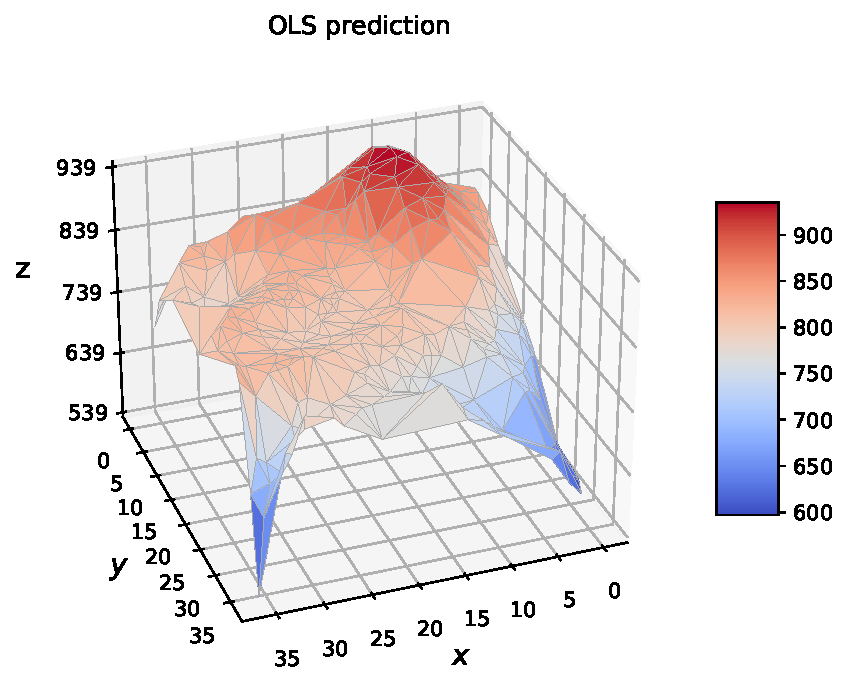
\includegraphics[width=\textwidth]{figures/OLS_predict_rd.pdf}
        \caption{Predictions of the test data for OLS method with $n=11$.}
    \label{fig:OLS_terrain_predict}
     \end{subfigure}
    \begin{subfigure}[b]{0.49\textwidth}
         \centering
         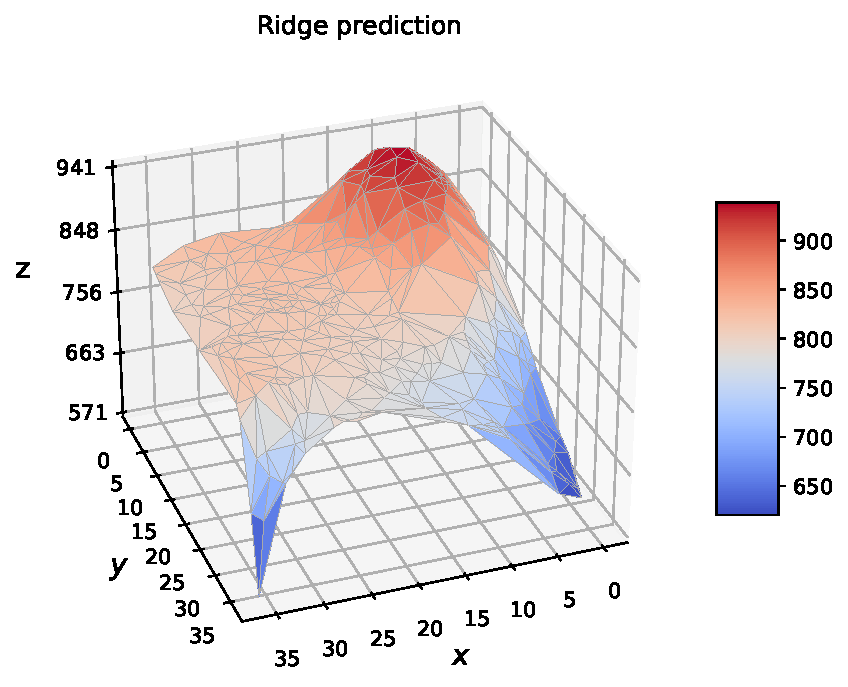
\includegraphics[width=\textwidth]{figures/Ridge_predict_rd.pdf}
          \caption{Predictions of the test data for Ridge method with $n = 12$ and $\lambda = \num{2.7e-10}$.}
          \label{fig:Ridge_terrain_predict}
     \end{subfigure}
     \hfill
     \begin{subfigure}[b]{0.49\textwidth}
         \centering
         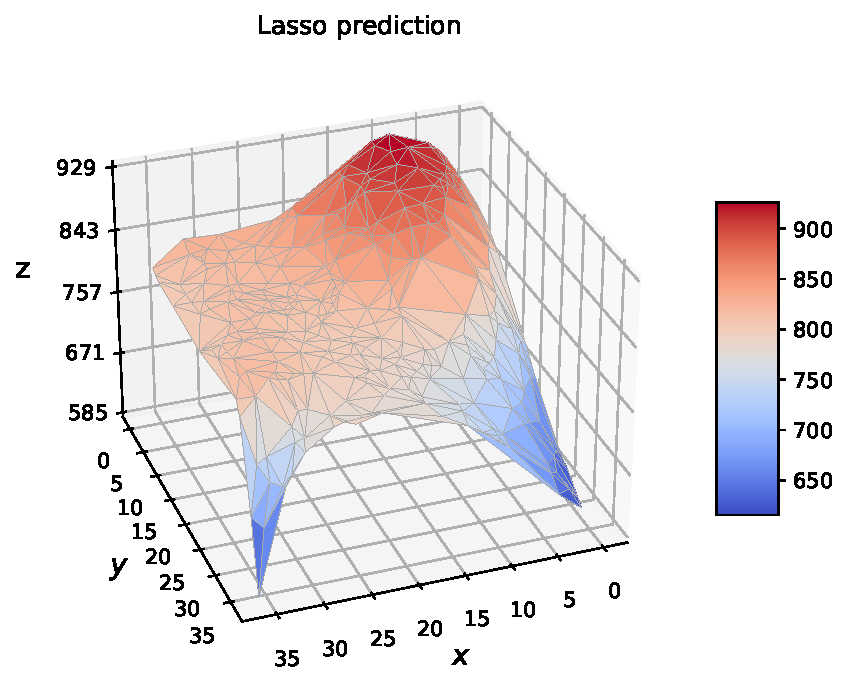
\includegraphics[width=\textwidth]{figures/Lasso_predict_rd.pdf}
         \caption{Predictions of the test data for Lasso method with $n = 19$ and $\lambda = \num{4.4e-7}$.}
        \label{fig:Lasso_terrain_predict}
     \end{subfigure}
    \caption{Comparing the predictions Subfigure}
    \label{fig:terrain_hyper_pred}
\end{figure}
From figure \ref{fig:terrain_hyper_pred} we observe visually that the predictions is replicate the trend of the test set fairly good. We compute the MSE error as shown in table \ref{tab:MSE_terrain_all_methods}.

\begin{table}[H]
  \begin{center}
  \caption{MSE score for the test data with methods; OLS, Ridge and Lasso. All methods using optimal values from training set.}
  \begin{tabular}{|c|c|c|c|} \hline
  & \text{OLS} & \text{Ridge} & \text{Lasso} \\\hline
  \text{MSE} & 0.06416 & 0.05698 & 0.07285  \\\hline
  \end{tabular}
  \label{tab:MSE_terrain_all_methods}
  \end{center}
\end{table}

From table \ref{tab:MSE_terrain_all_methods} we observe that the error is at the same order of magnitude with Ridge being slightly better than OLS which comes out slightly better than Lasso. This is somewhat similar to the results found with Franke's function. 


When calculating the optimal hyperparameters, we found that the result was quite sensitive to how the data was split into train and test for each trial. Even when keeping the choice of optimal hyperparameters fixed we still got a lot of variation in the test MSE on a magnitude of roughly $\pm 0.05$. Thus we cannot really compare which of the models performs the best for the terrain data, but since the $\lambda$-value was relatively low for both Ridge and Lasso we might conclude that OLS is a fairly good model. The reason for the variation from trial to trial can be explained by the randomness associated with the train-test-split. Since we only have 289 data points we quite easily risk that the data is unevenly distributed on the domain, and thus the modelling of the data will naturally differ. \\
Regarding the accuracy of the hyperparameters we refer back to the discussion done in section \ref{sec:franke_model}, as this is analog for this as well.\\
\end{document}
